%Dear all,
%We ar writing to invite you to submit an article to an upcoming special issue of the journal Hippocampus with the tentative title: Computational models of the hippocampus and related structures.  The theme includes computational and theoretical models as well as theory-driven data analysis of the hippocampus and related cortical and sub-cortical structures. 
%
%Articles for the special issue will be due June 15, 2019 with a planned publication date in early 2020.  All articles will be published on-line when accepted, but we will need to be firm about the deadline in order to avoid delays in publishing the full issue with volume and page numbers.
% 
%
%The contributions to the special issue can be in all forms of manuscripts accepted by Hippocampus (Commentaries, Reviews, Articles, Rapid Communications).
% 
%
%As is common with these types of special issues, we ask that any contributing author commit to reviewing two articles for the special issue.
% 
%
%Please let me know by Dec. 15 if you plan to contribute to this special issue.  Please also send me a tentative title and potential author list (which can change later if necessary).
%
%Best regards,
%Michael Hasselmo
%and Ehren Newman


\documentclass[11pt, titlepage, twoside]{article}
\usepackage[top=20mm, bottom=20mm, left=20mm, right=20mm]{geometry}
\geometry{a4paper}
\geometry{portrait}
\usepackage[utf8]{inputenc}	% Comment out for xelatex; must use with pdflatex
\usepackage[T1]{fontenc}
\usepackage[parfill]{parskip} % Activate to begin paragraphs with an empty line rather than an indent
\usepackage{graphicx}
\usepackage{amsmath}
\usepackage{amssymb}
%\usepackage{fontspec}
\usepackage{epstopdf}
\usepackage{float}
\usepackage[hang]{footmisc}
\usepackage{endnotes}
\usepackage{listingsutf8}
%\restylefloat{table}
\usepackage{xcolor}
\usepackage{colortbl}
%\usepackage{booktabs}
\usepackage{tabu}
\usepackage{caption}
\usepackage{textcomp}
\usepackage{textgreek}

\usepackage{subcaption}

% !BIB TS-program = biber
\usepackage[british]{babel}
\usepackage{csquotes}
\usepackage[style=apa]{biblatex}
\DeclareLanguageMapping{british}{british-apa}

\addbibresource{references.bib}
\usepackage{longtable}
\usepackage{csvsimple}				% for reading cvs files into tables

\makeatletter
\def\blx@maxline{77}
\makeatother

\captionsetup[figure]{labelfont=sc}
\captionsetup[table]{labelfont=sc}
\captionsetup[tabu]{labelfont=sc}

\DeclareCaptionType{MPEquation}[][List of equations]
\captionsetup[MPEquation]{labelformat=empty}

\DeclareCaptionType{MPListing}[][List of listings]
\captionsetup[MPListing]{labelformat=empty}

\usepackage{fancyhdr}
\setlength{\headheight}{16pt}
\pagestyle{fancyplain}
\fancyhf{}
%\fancypagestyle{plain}{}
\cfoot[\thepage]{\thepage}

\usepackage{stringenc}
\usepackage{pdfescape}


% Helper for debugging pdflatex errors induced by invalid UTF8 characters:
% output the actual character code causing the issue.

\makeatletter
\renewcommand*{\UTFviii@defined}[1]{%
\ifx#1\relax
\begingroup
% Remove prefix "\u8:"
\def\x##1:{}%
% Extract Unicode char from command name
% (utf8.def does not support surrogates)
\edef\x{\expandafter\x\string#1}%
\StringEncodingConvert\x\x{utf8}{utf16be}% convert to UTF-16BE
% Hexadecimal representation
\EdefEscapeHex\x\x
% Enhanced error message
\PackageError{inputenc}{Unicode\space char\space \string#1\space
(U+\x)\MessageBreak
not\space set\space up\space
for\space use\space with\space LaTeX}\@eha
\endgroup
\else\expandafter
#1%
\fi
}
\makeatother

% Make multi-paragraph footnotes align nicely on the left
\setlength\footnotemargin{10pt}

% Do not display an automatic Notes heading for endnotes, as they are contained
% by a Manuscripts section with a heading that has possibly been edited by the user
\def\enoteheading{}

% Apply footnote and endnote numbering schemes (decimal, lowercase roman etc.)
\renewcommand{\thefootnote}{\arabic{footnote}}
\renewcommand{\theendnote}{\arabic{endnote}}
% Adjust endnotes to use normal-sized numbering and text
\renewcommand{\enotesize}{\normalsize}
\renewcommand\enoteformat{%
  \raggedright
  \leftskip=1.8em
  \makebox[0pt][r]{\theenmark. \rule{0pt}{\dimexpr\ht\strutbox+\baselineskip}}%
}

\renewcommand*{\thefootnote}{\fnsymbol{footnote}}

\usepackage{xr}
\externaldocument{supplemental}

\begin{document}
\title{Complementary roles of Theta and Alpha in Multi-Item Associations}
\author{Nicholas Ketz\textsuperscript{1}\footnote{Nicholas Ketz current affiliation is: Information and Systems Sciences Lab, HRL Laboratories, Malibu, CA 90265}, Tim Curran\textsuperscript{1} and Randall C. O'Reilly\textsuperscript{1}}
\date{
	\textbf{1} Department of Psychology and Neuroscience, University of Colorado Boulder  
	 \\
	\today
}

\maketitle


%\section*{Acknowledgements}\label{sec:acknowledge}


\section*{Abstract}\label{sec:abstract}
%The Abstract should be clearly written in 300 words or less and should succinctly state the objectives of the study, experimental design, major observations and conclusions, and their major significance. The abstract should be intelligible to neuroscientists in general and should thus be free of specialized jargon and abbreviations. References should generally not be cited in the abstract, but if they are, the complete citation should be given. Please provide main keywords.
Through the use of neural network models of the hippocampus and surrounding cortex this work proposes a framework for understanding how time frequency signatures measured at the scalp can be used to track declarative memory processes, and make quantitative predictions about how information stored in long term memory is altered by these processes.  The fundamental hypothesis explored here is that neural oscillations in the theta (3-8 Hz), and alpha (8-12 Hz) frequency bands can be tied to specific neural mechanisms supporting declarative memory, and that these oscillatory signatures can be tracked in human scalp EEG recordings to predict behavioral changes in declarative memory processes. Specifically, oscillatory power in the theta band positively correlates with the how much information the hippocampus is reactivating for a given retrieval event, and that power in the alpha band positively correlates with how much information is being inhibited from being retrieved.  We first explore this idea through computational simulations of thalamo-cortical-hippocampal interactions which make a series of predictions tested in a human EEG experiment using the Dependent Events paradigm.  Results largely support the idea that thalamically mediated changes in alpha power during episodic memory encoding and retrieval are related to the flow of information between the neocortex and hippocampus, and that the bandwidth of this information flow tracks with theta power.  Further, this model suggest the encoding and retrieval processes are inter-dependent and that attentional modulation of what gets retrieved from long term memory subsequently impacts the information that is encoded into the underlying representation.

\section*{Keywords}
%Please provide up to 5-7 keywords. Keywords should be taken from those recommended by the US National Library of Medicine's Medical Subject Headings (MeSH) browser list at www.nlm.nih.gov/mesh.
Episodic Memory, Brain Waves, Neural Networks, Thalamus, Hippocampus


\section{Introduction}\label{sec:intro}

It is generally accepted that long-term memory encoding and retrieval are not isolated functions of any one brain area \cite{Gabrieli98,PrinceDaselaarCabeza05}.  However, there are many challenges in moving beyond the traditional studies focusing on individual regions  (e.g., concentrating on the prominent role of the hippocampus), to obtain insight into the nature of network-level dynamics.  An increasing body of work support the idea that oscillatory dynamics in multiple brain regions are associated with different aspects of  memory encoding and retrieval \cite{NyhusCurran10,HanslmayrStaudiglFellner12,Klimesch12}, %update refs here!!!
These studies have generally found a consistent relationship between several frequency bands and successful encoding or retrieval of experiences; namely that oscillatory power within the alpha (8 to 12Hz) and beta (13 to 30Hz) frequency bands generally decrease with the successful execution of these memory processes, while theta (3 to 8Hz) and gamma (30 to 100+Hz) increase in the regions directly involved in the memory operations. Why these relationships exist, and what they tell us about the larger functional organization of memory systems in the brain are still open questions.
 
One model suggests that thalamic circuits play a functional role in selectively gating communication between cortical regions by synchronizing them in various frequency bands \cite{ShermanGuillery06,SaalmannKastner11,KetzJensenOReilly15}.  These gating mechanisms, implemented  by oscillatory synchronization, are central to system level brain function and ultimately affect cognitive behavior such as memory encoding and retrieval.  Further, the particular oscillatory dynamics engaged by this selection process may provide indicators of which system-scale neural circuits are coordinating together to facilitate that particular form of memory processing.

A particular thalmo-cortical circuit of interest for memory processes involves the hippocampus and its associated subcortical network, including the anterior thalamus, and medial septum which are essential in the maintenance of theta oscillations (4 to 8 Hz) \cite{Buzsaki02}.  Theta oscillations have been shown to be critically involved in successful encoding and retrieval of episodic like memories in both humans and animals \cite{NyhusCurran10,JonesWilson05,FuentemillaBarnesDuzelEtAl14}, and are believed to be primarily driven by the pacemaker cells within the medial septum.  The anterior thalamus, however,  provides the connectivity for the hippocampus to potentially modulate communication with the medial and orbital PFC through theta synchronization \cite{VanderWerfJollesWitterEtAl03,AggletonDumontWarburton11}.  Thus, the theta circuit is important for the core functioning of the hippocampus during encoding and retrieval.

%There is MEG evidence that theta synchronization with the hippocampus can facilitate Recollective memory processes in humans \cite{FuentemillaBarnesDuzelEtAl14}. There is some indirect MEG and BOLD evidence that the thalamus plays a role in this synchronization process \cite{FuentemillaBarnesDuzelEtAl14,PergolaRanftMathiasEtAl13}, which is bolstered by the known connectivity between the hippocampus and PFC through the anterior thalamus from rodents \cite{AggletonBrown99,AggletonDumontWarburton11}.  The thalamic gating model connects these ideas suggesting Recollective memory works through the hippocampus via theta synchronization, however to date there is no strong evidence supporting this claim in humans.

A complimentary thalamic circuit involves the pulvinar providing synchronization within the alpha (8 to 12 Hz) band between parietal and visual cortices with the medial, orbital and lateral PFC \cite{BarbasHenionDermon91,KievitKuypers77,LopesdaSilva91}.  This circuit is important for bottom-up stimulus-driven encoding processes in memory \cite{JutrasFriesBuffalo13}, but it can also inhibit contradictory or interfering information during internally guided retrieval \cite{ParkLeeKangEtAl14}.  Thus, its overall contribution to memory can be mixed, and depends on the nature of the task and what kinds of memory processing is required.

%The pulvinar has a well established role in coordinating alpha synchrony in animal models \cite{SaalmannKastner11,SaalmannKastner09,LopesdaSilva91,LopesdaSilvaVosMooibroekEtAl80}, and there is recent evidence in human models showing alpha oscillations provide an active function of suppressing cortex that would otherwise interfere with the memory retrieval \cite{WaldhauserJohanssonHanslmayr12,HanslmayrStaudiglAslanEtAl10,KhaderRosler11}.  There is also human fMRI evidence showing PFC modulation of visual cortex through the pulvinar \cite{SotoHumphreysRotshtein07,RotshteinSotoGrecucciEtAl11}.


Indeed, a recent spiking model of these oscillations called the Sync/deSync Model highlights the role of a synchronized hippocampus that accompanies a desynchronized neocortex during encoding and retrieval.  This model in particular focuses on the role of decreased alpha power related to successful encoding of new information \cite{ParishHanslmayrBowman18, HanslmayrStaresinaBowman16}.  Similarly, recent empirical studies of human intracranial recordings find evidence to support the complimentary roles of hippocampal synchrony and neocortical desynchrony in successful encoding and retrieval \cite{GriffithsMichelmannRouxEtAl18, StaresinaMichelmannBonnefondEtAl16}.  In general these results find a decrease in neocortical alpha power and an increase in hippocampal gamma power that coincide with successful encoding and retrieval of declarative memories. 


This accumulated evidence suggests a relationship between theta and alpha frequency bands and long-term memory systems as constructed by the Complimentary Learning Systems theory \cite{McClellandMcNaughtonOReilly95,OReillyBhattacharyyaHowardEtAl14}.  Namely, that theta power positively tracks successful engagement (encoding/retrieval) between hippocampus and neocortex, while alpha power negatively tracks with this process as active inhibition of cortex is released in response to the exchange of information between hippocampus and neocortex.  This relationship is further supported by the connectivity of the thalamus with cortex such that a specific model for how information is routed into and out of these systems can be tied to empirical measures of neural oscillations.  This work seeks to test this relationship through a series of computational simulations of hippocampal-thalamo-cortical interaction, and an accompanying EEG study in humans to compare against simulation results.

In general, our results show that our model can capture broad time frequency dynamics related to alpha and theta oscillations, and that it can be used to evaluate patterns of human EEG against an underlying theoretical model.  This model provides explanatory power in understanding how thamalmo-cortical attentional mechanisms can enhance the binding between multi-item associations through reactivation, as well as diminish those associations when the underlying encoding structure does not promote reactivation.  


\subsection{Dependent Events Paradigm}
%
%Hippocampal dependent memory is generally thought to be associative in nature, where multiple cortical representations are bound together in a distinct hippocampal representation during encoding.  Later, an incomplete set of those cortical representations can be used as a cue to reactive the full set during retrieval \cite{McClellandMcNaughtonOReillyEtAl92}.  This multi-element type of memory retrieval is also referred to behaviorally as `Recollection' where multiple details of a given experience can be retrieved, and hippocampal activity increases with subjective confidence and the amount of information being retrieved \cite{RuggVilbergMattsonEtAl12}.  
%
%In contrast to Recollection, memories that exhibit `Familiarity' have no measurable details that can be recalled, however individual elements can be successfully recognized when presented with a mix of lures.  This Familiarity process is thought to rely more heavily on the medial temporal lobe (MTL) cortex surrounding the hippocampus, including entorhrinal, parahippocampal, and perirhinal cortices.  These cortical areas, among others, are proposed to be a separate memory system from the hippocampus, serving behavior when recall of all associated details is not necessary or available \cite{EichenbaumYonelinasRanganath07,AggletonBrown99}.  This theory of separate memory systems has been contentious for several decades with evidence both in support and in contrast to its core ideas  \cite{EichenbaumYonelinasRanganath07,WixtedSquire10}; namely that Recollection can occur in addition to Familiarity and that the hippocampus is not specific to Recollection but can be used in Familiarity based processing.  What is clear is that MTL cortex learns and maintains representations required for hippocampal retrieval, and those MTL regions along with the hippocampus can be used to re-instantiate cortical representations outside MLT during retrieval \cite{RuggVilberg13}.  
%

\begin{figure}
    \begin{center}
	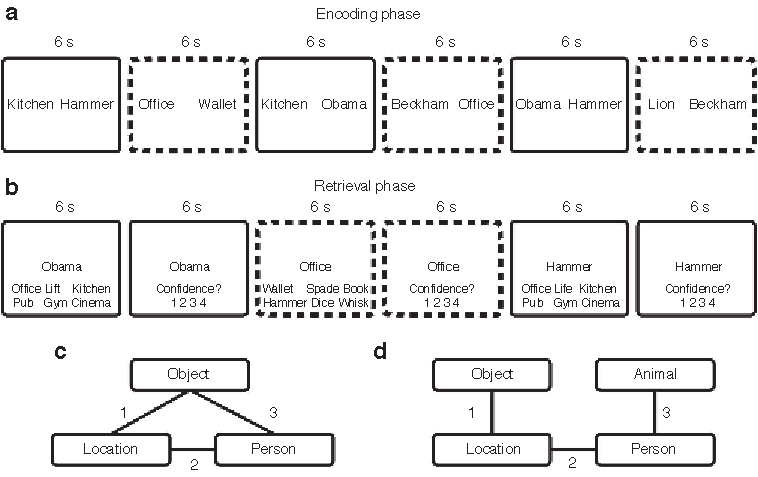
\includegraphics[width=.9\textwidth]{figs/deev.pdf}
    \end{center}
      \caption[Dependent Events Paradigm]{
       Dependent events behavioral paradigm, taken from \textcite{HornerBisbyBushEtAl15} (a) Encoding phase. Participants see multiple paired associates and imagine each pair `interacting in a meaningful way as vividly as possible' for 6 s. Solid lines and dotted lines were not present, but highlight a closed-loop (solid lines) and open-loop (dotted lines) event. (b) Retrieval phase.  Participants were presented with a single cue and required to retrieve one of the other elements from the same event from among five lures within 6 s. This was followed by a 1-4 confidence rating within 6 s.  All 6 possible cue-target combinations are tested (c) The associative structure of closed-loop events, with example encoding order for the three pairwise associations (numbers 1-3). (d) The associative structure of open-loop events, with example encoding order for the three pairwise associations.
	}
     \label{fig:deev}
\end{figure}


To test this inverse relationship between theta and alpha we choose a recent hippocampal dependent multi-item association study to base our computational and empirical investigations on \cite{HornerBisbyBushEtAl15} (see Figure \ref{fig:deev}).  In this study the authors used a previously developed paradigm (see \textcite{HornerBurgess13,HornerBurgess14}) in which they manipulated the binding of a set of overlapping paired associates.   Here two types of associative stimuli were studied, closed-loop and open-loop. In the `closed-loop' events participants studied a set of paired associates on separate trials, e.g. Person-Location, Location-Object, and Object-Person, where each category refers to the same stimulus for a given event.  This created a complete set of binding between all elements.   In contrast, the `open-loop' events incorporated a new element and left some relationships unstudied, e.g. Object-Location, Location-Person, Person-Animal.  Each of the associations was later tested in a cued recognition task, which showed greater inter-event Dependency for the closed-loop compared to the open-loop associates.  Dependency here is operationalized as the retrieval of \emph{all} associated pairs from a given event, or none; whereas no Dependency would imply retrieval of some of the associated pairs but not all.  The goal of this metric is to capture the strength of the binding between elements within a given event, where high Dependency indicates strong associations leading to retrieval of all items within a given event, and low Dependency indicates weak associations leading to some of the items being retrieved incorrectly. In contrast, a non-associative measure of accuracy can be made using an Independent model which calculates Dependency based on the assumption that each retrieval trial is statistically independent from the next, see Section \ref{sec:CalcDep} for more details.  %This provides a nice measure of both Recollection yielding high Dependency from strong associations between elements, but also uses a recognition paradigm where successful retrieval with low between element Dependency implies a similar construct to Familiarity, i.e. retrieval without detailed recall.

%theta increase a marker of hippocampal retrieval (Nyhus and Curran, 2010), and should correlate with amount of cortex reinstated
In this paradigm, closed-loop events show significantly greater Dependency as compared to the Independent model while the open-loop events showed no difference compared to its Independent model, implying that closed-loop events have a stronger between element binding as compared to open-loop events.  The closed-loop condition also showed more cortical reactivation of non-target elements within an event (i.e. studied elements not currently the target of the recognition trial), and that this reactivation correlated with hippocampal activity.  Results from fMRI studies such as \textcite{HornerBisbyBushEtAl15} provide spatially specific evidence for the hippocampus driving cortex to reinstate previous studied elements, but provide no evidence relating these processes to potentially related neural oscillations.  A computational model tied to the neural oscillations of this phenomena can provide an opportunity to bring clarity to this relationship by testing if patterns in theta power can be predicted by a computational model of the hippocampus.  Key aspects, however, relating to the focus of attention and alpha power are required to adequately model the paired associate and cued recalled components of the Dependent Events paradigm.



\subsection{Theta-Phase Model}

Building off our previous connectionist model of the hippocampus \cite{KetzMorkondaOReilly13}, referred to here as the Theta-Phase model, we seek to incorporate the ability to attend to particular dimensions of a given input pattern, while not attending to others.  Practically, this requires that each input be described on all possible stimulus dimensions, otherwise the hippocampal model will attempt to `recall' the missing information for those missing dimensions.  For example, one valid cortical representation experienced will contain information about size and shape but never in color, while another equally valid representation will contain information about color and shape, but never size.  The neural substrate supporting these representations needs to be able to represent all three dimension (and potentially many others) simultaneously and independently, but also be able to understand the inherent bias in which dimensions are likely to covary together.  

%This problem begins to touch on the issue of intentional vs. incidental retrieval.  Intentional retrieval implies a goal directed, attentionally mediated re-activation of previously experienced representations, while incidental retrieval implies the reactivation of representations that are likely to be experienced together.  The Theta-Phase model is built exclusively on incidental retrieval mechanisms and currently has no way of reflecting the attentional, or goal directed, focus of the retrieval process.  Similarly, the lack of an intentional component to the retrieval process requires the Theta-Phase model to have valid, useful information in all potential stimulus dimensions, which is simply not possible in every scenario.  However, it is also crucial to maintain this incidental component to the model as it is fundamental to the Complimentary Learning Systems theory, and the main mechanism behind pattern completion \cite{McClellandMcNaughtonOReillyEtAl92,NormanOReilly03}.  What is required is an ability to balance between intentional and incidental retrieval drives in such a way that fits with known behavioral patterns.

A simple and ecologically valid way to reconcile this discrepancy is a mechanism that would highlight which of the stimulus dimensions are informative, or relevant given the current input.  This would be very similar to a selective attention mechanism.  Building from the evidence in support of an alpha mediated thalamic gating mechanism, we will explore modulation of cortical activity via thalamo-cortical interactions in the alpha band as a mechanism for the Theta-Phase model to gate specific stimulus dimensions for targeted encoding and retrieval.  The behavioral and physiological consequences of this mechanism will then be explored in a long-term memory paradigm that utilizes multi-element traces, and a bottom-up attentional signal to focus on specific stimulus dimensions.


\subsubsection{Attention and Alpha Oscillations}
\textcite{ShermanGuillery06} provide the most complete framework for how the flow of information can be guided from low level sensory regions into higher level cortical regions best suited for task specific processing.  The simple yet compelling idea is that cortical-cortical projections convey the contentful output from a given cortical region, while the thalamo-cortical projections contain the gating information.  Sensory information is allowed to cascade from one processing region to the next through cortical-cortical projections, provided that a selective thalamo-cortical gating signal alerts/allows the next cortical region to accept (or block) the incoming cortical-cortical signal.  

The other critical aspect of this bottom-up attention mechanism is the connection to alpha oscillations.  Historically, alpha power has been shown to correlate with the onset of sleep, which led to the suggestion that high alpha power indicates an idle or perhaps inhibited cortical region.  The mechanistic connection between alpha power and thalamic gating is captured in the firing properties of the thalamic relay cells (TRC) which show two distinct modes of firing.  The first shows oscillatory firing patterns acting like a pacemaker system in the alpha frequency range (approximately 10 Hz or 100ms periodicity), and is generally referred to as bursting.  This bursting mode is believed to be engage when a given cortical region is in an idle state, i.e. when no active processing is occurring in the thalamus or the corresponding cortex linked to that thalamic relay region.  The other regime, referred to as tonic firing, shows no specific oscillatory firing pattern, and instead shows increased spontaneous firing in both the thalamus and corresponding cortical regions \cite{LerescheLightowlerSolteszEtAl91,ShermanGuillery06,LopesdaSilva91}.  These dynamics have been studied extensively as a naturally occurring phenomena of thalamic interactions with cortex, however simulation studies have also shown the potential for these mechanisms to be used in a goal directed way \cite{HindriksvanPutten13,VijayanKopell12,LeeWhittingtonKopell13}. The implications of these results are that cortical regions being driving by TRCs in bust mode will show more alpha power, and will process the incoming cortical-cortical information less veridically, while cortical regions being driven by tonic TRC firing will show a relative decrease in alpha power and process cortical-cortical information more completely.  This is the foundation for the connection between alpha power and thalamic gating, such that increased alpha power is indicative of decreased cortical processing.

The detailed biology of this framework is well captured by \textcite{ShermanGuillery06}, and relies on two critical components not yet implemented in the Theta-Phase model: 1. The thalamic relay cells (TRC) that pass the gating signal onto the next cortical region, and 2. The cortical neurons in layers 5 and 6 that send this gating signal to the next TRC, and trigger the opening of the gate for processing in associated cortex for that TRC.  The following sections provides a high-level description of how these components are implemented, while supplementary info section \ref{appDeepLeabra} illustrates the detailed implementation into the LEABRA framework.


\begin{figure}
	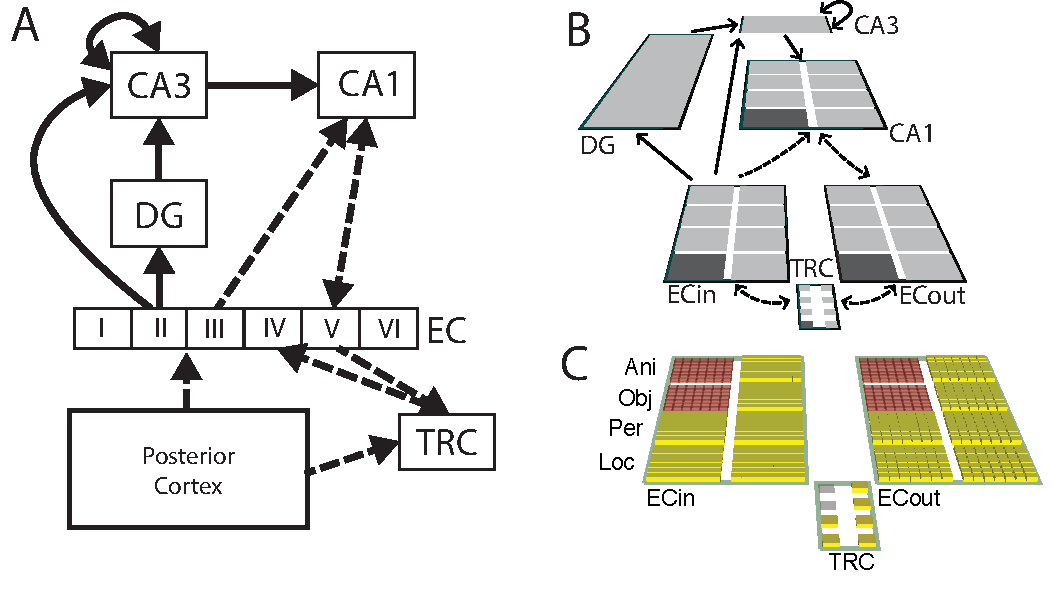
\includegraphics[width=\textwidth]{figs/depNet.pdf}
        \caption[Thalamic Gating as Implemented in Theta-Phase Model] {  \emph{(A)} Schematic of Theta-Phase model with thalamic gating.  Posterior cortex connects with both layers 2/3 of Entorhinal cortex (EC) via cortical-cortical projects, but also to thalamic relay cells (TRC) via layer 5 bursting cells.  These TRC units maintain their topography into EC layer 4 where they provide a gating signal for EC to accept or suppress the corresponding cortical-cortical projection. Topographic connectivity shown in dashed arrows, and distributed connectivity shown in solid.  \emph{(B)}  Neural network showing TRC implementation as single units for a given cortical area's input and corresponding unit group in EC.  This topography is kept consistent between TRC and EC unit groups.  \emph{(C)} Conceptualization of EC unit groups to paired associate elements and thalamic gating signal manifested in EC with 2 bottom-up cortical inputs missing (i.e. object and animal) in unit groups with a low (red) gating signal, and 6 inputs present (i.e. location, person, and 4 contextual elements) shown with a high (yellow) gating signal.  The cortical input topography is maintained between EC and TRC where TRC activation is used to calculate the normalized gating signal shown in the corresponding EC unit groups.  Note the gating signal is not representation specific, but rather generalized for a given unit group. 
        }
     \label{fig:depNet}
\end{figure}






\section{Computational Methods}\label{sec:compmethods}

In this work we start with the Theta-Phase model of the hippocampus and entorhinal cortex, as described in \textcite{KetzMorkondaOReilly13} and implemented in the Emergent framework \cite{AisaMingusOReilly08} (see Figure \ref{fig:depNet}).  Briefly, this model is built upon a series of structural and functional hypotheses based on anatomical and physiological data, which have been captured in the complementary learning systems (CLS) model of the hippocampus \cite{McClellandMcNaughtonOReilly95, NormanOReilly03}. The Entorhinal Cortex (EC) in the model is assumed to be the cortical gateway to the hippocampus.  This gateway feeds through the tri-synaptic pathway to the Dentate Gyrus (DG), CA3, and then to CA1.  Similarly, there is a parallel connection through the mono-synaptic pathway from the EC to the CA1 (and back).

The tri-synaptic pathway connections are broadly diffuse, and support the conjunctive binding of various distributed pieces of information into an overall episodic memory representation in the CA3. The mono-synaptic pathway conversely is topologically organized, not diffuse.  We capture this connectivity by organizing the simulated neurons in EC and CA1 into mutually interconnected {\em slots}, presumably encoding different separable elements/stimulus dimensions that loosely correspond to independent cortical regions converging on the EC \cite{Witter10}.  This slot architecture enables the mono-synaptic pathway to develop separable invertible pathways where a given EC input pattern can be encoded over a sparser representation in the corresponding CA1 slot, and this CA1 representation can in turn recover the full original EC slot pattern. 

The learning dynamics within this model, as governed by the LEABRA algorithm, are dictated by the phases of a presumed theta oscillation, thus its short-hand name of 'Theta-Phase' used here. In short, during learning two error signals are derived within every period of a give theta oscillation.  The first, during the trough of the theta oscillation, provides an error driven learning signal to the mono-synaptic pathway, learning the invertible mapping between EC and CA1 can be thought of as an encoding.  The second, during the peak of the theta oscillation, provides a error driven learning signal on the tri-synaptic pathway, learning to recollect missing or incomplete information can be thought of as retrieval.  

Building on this model that inherently captures the hippocampal theta dynamics, we seek to add a modulatory attention signal that can capture the appropriate alpha dynamics derived from the thalamo-cortical principles described above.  This following section reviews the specifics of that implementation, and the testing paradigm used to validate its performance.


\subsection{Thalamic Modulation as Alpha}
\label{sec:attmod}
The effective implementation of the selective attention mechanism into the Theta-Phase model is done through a separate layer that reflects the thalamic relay cell (TRC) activity, as well as an attentional modulation value calculated from this TRC activity that scales the net input of downstream units.  This can be seen implemented in the Theta-Phase model in Figure \ref{fig:depNet}.  Here connectivity between the posterior cortical inputs and Entorhinal Cortex (EC) also goes through a `TRC' layer corresponding to the thalamic relay cells that then supply the attentional modulation signal.  Each of the posterior cortical regions maintains topographic input into EC and the corresponding TRC, which is manifest in the model as separate unit groups as shown in Figure \ref{fig:depNet}B.  Each of these unit groups has a single TRC unit that calculates its modulatory signal as determined by the activation in the corresponding posterior cortical region and EC unit group.  Finally, a single modulatory scalar value is calculated for each of the TRCs and sent to its corresponding EC unit group either inhibiting activation in that unit group or allowing normal processing to occur. 

The detailed description of this modulator mechanism's implementation is described in supplementary info section \ref{appDeepLeabra}, however a coarse description and its functional implications are described here.  The attentional modulation is effectively a normalized scaling factor based on the net input to a given TRC unit.  A given TRC unit receives inputs with fixed weighted connections (i.e. no learning signal adjusts these weights), and its activation is used to calculate a single value that multiplicitively scales the net input of each of the units it is connected to.  This attentional scaling value is simply the TRC activation normalized to range from some pre-determined minimum to a maximum of 1.  This pre-determined minimum scaling factor can be thought of as the most inhibitory influence possible, and was loosely fit for these simulations to a value of 0.25 to match the anticipated accuracies across conditions.  It should be noted this minimum scaling value did not vary across trials or conditions and therefore is unable to bias reactivation. 


\subsection{Model Validation}
\label{sec:ModelTest}

The Dependent Events paradigm (see Figure \ref{fig:deev}) was chosen to test the performance of the combined Theta-Phase model with attentional gating.  This paradigm ideally captures behavioral components related to Complimentary Learning Systems ideas of pattern completion and separation, as well as components relating to selective attention over multi-element memory traces.  These two aspects allow for the testing of the computational model to match known behavioral performance and relate the findings to predictions in the EEG time frequency domain.

Basing the testing procedure off \textcite{HornerBisbyBushEtAl15}, the paradigm was implemented as close to the behavioral version as possible.  The model learned a series of multi-element `events', see Figure \ref{fig:deev}. Each event consisted of three or four elements (locations, people, objects and animals), plus 4 contextual elements that were consistent across presentations. Events were built up over three separate encoding trials (interleaved with encoding trials of other events). Each trial consisted of the presentation of one of the three possible pairwise associations from a given event. This paradigm allows for the building of `events' with different associative structures of overlapping pairs: `closed-loop', in which all event elements were presented paired with all other elements of the event; or `open-loop', in which elements of an event were presented as a chain of overlapping pairs. Here, the term `event' groups  the set of overlapping associations encoded across separate paired associate trials. 


The model's input patterns, described in more detail Section \ref{sec:HippModelValidation}, were created with a base vocabulary of 100 7x7 unit group patterns with 7 units active and a minimum Hamming distance of 10 between each pattern.  The composite input patterns used to train the model were generated from this set of vocabulary patterns, with 8 unit groups in each input pattern.  These input patterns were conceptualized to have 4 unit groups that each corresponded to one of the various element types of the paired associates used in the Dependent Events paradigm.  For each event, one unit group had a unique pattern of activity that corresponded to `location' representations, another for `people', another for `objects', and another for `animals'.  These patterns were consistent across presentations of a given event, i.e. the same unit group patterns were used across the 3 encoding trials, and 6 retrieval trials for each event. In this way selective attention during encoding and retrieval can be  guided to these specific stimulus dimensions of the input pattern, as shown in Figure \ref{fig:depNet}C where two element types are being presented and the corresponding attentional modulation signals are being shown inhibiting the non-attended dimensions.  In addition to these 4 unit groups corresponding to the different event element types, 4 incidental unit groups also maintained the same representation across event presentations.  This was conceptualized as other contextual elements of the event participants imagined, and likely aided in the model's ability to recall the associations (although simulations without these contextual elements were not explored). 

\subsection{Testing Procedure}
\label{sec:TestProc}
The encoding phase was split into three mini-blocks. One pairwise association for each of the 36 events was presented during each of the three mini-blocks. Presentation order within each mini-block was randomized. For the closed-loop events, the order of presentation across the three mini-blocks for a specific event was either: (1) location-object/animal, location-person and person-object/animal, (2) person-object/animal, location-person and location-object/animal, (3) location-person, location-object/ animal, person-object/animal or (4) location-person, person-object/animal and location-object/animal. For open-loop events, it was either: (1) location-object, location-person, person-animal, (2) person-animal, location-person, location-object, (3) location-person, location-object, person-animal or (4) location-person, person-animal, location-object. Each of the four orderings was run on two random initialization of weights, to make up the pool of results. The model was trained on 2 epochs (random permutations of all the trials within a mini-block) for each mini-block before starting training on the next mini-block.  Thus, for the first and second mini-blocks, the closed-loop and open-loop conditions were identical, presenting a single pairwise association and then a second overlapping pairwise association. In contrast, the third mini-block either formed an all-to-all associative structure in the closed-loop condition or an associative chain in the open-loop condition as shown in Figure \ref{fig:deev}.

At retrieval, the model was tested on each encoded pairwise association for each event in both directions.  In this way, each event was tested across six separate retrieval trials.  In the behavioral paradigm each retrieval trial was a six-forced choice recognition test with a particular cue element type and potential 6 targets all from the same element type (for example, cue location, retrieve the associated person among five people from other events).  However, in the model, this was captured by providing an activation of 0.1429 to all units in the target element dimension, providing a similar net activation compared to the complete patterns (i.e. $49 * 0.1429=7$), and thus opening the thalamic gate to allow processing in the target dimension. Note that a single cue pattern, and non-informative target dimension activation were presented on all retrieval trials with the task being to reactivate the original paired associate.  This reactivation success was measured by the binary Name Error metric described in Section \ref{sec:HippModelValidation}, i.e. either correct reactivation or not for a given cue-target pair. Thus, as with encoding, the closed-loop and open-loop conditions were exactly matched in terms of stimuli and task demands, differing only in the potential occurrence of incidental reactivation (that is, different levels of pattern completion).  
%An example of what this looks like in the network is shown in Figure \ref{fig:netNonTarg}B, with more pattern completion occurring in the location stimulus dimension (both in ECout and the TRC layer) for the closed-loop condition compared to open-loop.

Two parameters were loosely fit to match retrieval performance from previous behavioral results of the Dependent Events paradigm \cite{HornerBisbyBushEtAl15,HornerBurgess14}.  The first was the number of training repetitions (referred to as `epochs') for each mini-block of encoding.  The second was the minimum amount of attentional modulation, i.e. when the thalamic gate is fully closed how much activation is allow to get through, see Section \ref{sec:attmod} and Appendix \ref{appDeepLeabra} for more details.  By coarsely comparing results from Name Error determined retrieval accuracy in the network, shown in Figure \ref{fig:netDep}, to the known behavioral results from \textcite{HornerBisbyBushEtAl15,HornerBurgess14}, the two parameters were fit (2 epochs of training per mini-block, and a minimum activation of 0.25) to loosely match network performance with human behavior.

\subsection{Measure of Event Dependency} 
\label{sec:CalcDep}
Based on \textcite{HornerBisbyBushEtAl15}, dependency between event elements was assessed by constructing contingency tables for successfully retrieving, on separate trials, the two associated elements (for example, person and object) when cued by the remaining element (for example, location), as well as for retrieving a particular target element (for example, location) when cued by the other two elements (for example, person and object), see Table \ref{tab:depEvt} for example contingency tables. Averaging across events within conditions, this resulted in six 2x2 tables per model run per condition with the on-diagonal elements reflecting the Dependency for a given cue or target element.  These were then averaged across the 4 contingency tables with shared associations across both open and closed loop conditions (i.e. location and object cue and target tables) to get a single measure of dependency per condition.

To accurately compare condition differences in Dependency between open and closed-loop events its necessary to control for accuracy differences.  For example, if all paired associates are correctly retrieved it's unclear if there is inherent Dependency between event elements or if each association was memorized independently.   To address this, an `Independent' model that reflects the expected Dependency irrespective of the underlying event structure can be calculated to compare with the Dependency inherent in the event structures. For a given model random weight initialization, the mean proportion of correct retrievals for a given element type, say $B$, (over all events) when cued by a given element type, $A$ , can be denoted as $P_{AB}$. This accuracy can be used to create contingency tables for an Independent model where the probability of correctly or incorrectly retrieving two associations is simply the product of the mean probability for each association (i.e., the proportion of events for which both $B$ and $C$ were correctly retrieved when cued by $A$ would be $P_{AB}  P_{AC}$, while the proportion where $B$ was correctly retrieved but $C$ was not would be $P_{AB}(1-P_{AC})$).  A example contingency tables for the Independent model are show in Table \ref{tab:depInd}.


\begin{table}
\parbox{.45\linewidth}{
\centering
\begin{tabular}{l | c c}
	Cue$_{A_i}$ & Hit$_{C_i}$ & Miss$_{C_i}$ \\
	\hline
	Hit$_{B_i}$ & $H_{A_i B_i} \land H_{A_i C_i}$ & $H_{A_i B_i} \land M_{A_i C_i}$\\
	Miss$_{B_i}$ & $M_{A_i B_i} \land H_{A_i C_i}$ & $M_{A_i B_i} \land M_{A_i C_i}$\\	
	\hline
\end{tabular}
\newline
\vspace{5mm}
\newline
\begin{tabular}{l | c c}
	Targ$_{A_i}$ & Hit$_{C_i}$ & Miss$_{C_i}$ \\
	\hline
	Hit$_{B_i}$ & $H_{B_i A_i} \land H_{C_i A_i}$ & $H_{B_i A_i} \land M_{C_i A_i}$\\
	Miss$_{B_i}$ & $M_{B_i A_i} \land H_{C_i A_i}$ & $M_{B_i A_i} \land M_{C_i A_i}$\\	
	\hline
\end{tabular}
%\vspace{5mm}
\caption[Contingency Tables for Data driven Dependency]{Contingency tables for a given event $i$ focused on element $A$.  $H_{A_i B_i }$ implies a correct retrieval with cue element $A$ and target element $B$ from event $i$, while $M_{A_i B_i}$ implies an incorrect retrieval with the same cue and target, $\land$ implies a logical and. \label{tab:depEvt}
}
}
\hfill
\parbox{.45\linewidth}{
\centering
\begin{tabular}{l|cc}
	Cue$_{A}$ & Hit$_{C}$ & Miss$_{C}$ \\
	\hline
	Hit$_{B}$ & $P_{AB} P_{AC}$ & $P_{AB} (1-P_{AC})$ \\
	Miss$_{B}$ & $(1-P_{AB}) P_{AC}$ & $(1-P_{AB}) (1-P_{AC})$ \\	
	\hline
\end{tabular}
\newline \vspace{5mm} \newline
\begin{tabular}{l|cc}
	Targ$_{A}$ & Hit$_{C}$ & Miss$_{C}$ \\
	\hline
	Hit$_{B}$ & $P_{BA} P_{CA}$ & $P_{BA} (1-P_{CA})$ \\
	Miss$_{B}$ & $(1-P_{BA}) P_{CA}$ & $(1-P_{BA}) (1-P_{CA})$ \\	
	\hline
\end{tabular}
\caption[Contingency Tables for Independent Dependency]{Independent model contingency table focused on element $A$ across all events.  $P_{AB}$ implies percent correct across all retrieval trials where element category $A$ is the cue and element category $B$ is the target. \label{tab:depInd} 
}
}
\end{table}


\section{Behavioral and EEG Methods}\label{sec:behmethods}


\subsection{Participants}
49 University of Colorado undergraduates participated in the experiment and received payment of \$15 per hour (ages 18-29, mean$=$19.76; 30 male, 19 female). All participants were right handed, had normal or corrected-to-normal vision, and all but 5 were native english speakers.  Informed consent was obtained from each participant, and the study conformed to the Human Research Committee guidelines.  Two participants were removed due to equipment malfunction, nineteen were removed due excessively noisy EEG data such that they had less then 20 trials in any experimental condition.  This excessive number of participants removed based on low trial counts is likely due to two factors: first is the paradigm requires participants to move their eyes, causing more EEG artifacts then would be expected otherwise, and second is the sub-selection of trials by correctness and confidence as discussed in Section \ref{sec:deevEEGConf}.  

\subsection{Materials}
Experimental stimuli, originally adapted from \textcite{HornerBisbyBushEtAl15}, were 252 individual words split into 4 categories with 72 locations, 72 people, 54 objects, and 54 animals.  72 individual `events' were generated for each participant, half of which were closed-loop events consisting of three elements (e.g. location-person-object), and half were open-loop events consisting of 4 elements.  Half of the closed-loop events consisted of location-person-object triplets and half consisted of location-person-animal triplets.  These 72 events were equally split into two blocks balancing across all event types, and the subset of words used to generate events in block 1 was the same across participants.  An example set of events for block 1 is shown in Appendix \ref{appStimuli}.  

Stimuli were presented on a 17-in flat-panel display with a resolution of 1024 $\times$ 768 (60 Hz frame rate) placed approximately 1 m in front of the participants. Words were presented in 30 point Geneva font.  All portions of the display not occupied by stimuli or text were filled with white pixels. The experiment was programmed in MATLAB (versions R2012b and R2014a; The MathWorks, Inc., Natick, MA) and was presented using Psychtoolbox \cite{Brainard97}.  Mixed effect statistical analysis was done using R 3.2.1, and the lme4 package version 1.11-11 \cite{BatesMachlerBolkerEtAl14}.  Significance values for mixed effect models were estimated using the Satterthwaite approximation for degrees of freedom, using the lmerTest package version 1.0.


\subsection{Design}
The experiment consisted of 2 blocks of 2 experimental phases (as shown in Figure \ref{fig:deev}): paired associate encoding, and cued recognition. Each session, including application of the electrode net and performing the task, lasted approximately 2 hours. Stimuli were subdivided into 2 blocks such that there were 18 unique open-loop events per block and 18 closed-loop events per block.  Each of the open-loop events consisted of a unique location-person-object-animal quadruplet of words, and half of the closed-loop events consisted of a unique location-person-object triplet of words and the other consisted of a unique location-person-animal triplet of words.  

Each of these events were presented in pairwise association during the paired associate encoding phase.  The encoding phase was split into three mini-blocks such that one pairwise association for each of the 36 events was presented during each mini-block. Presentation order of events within each mini-block was randomized. Presentation of association pairings across mini-blocks for a specific event was done in 1 of 4 ways dictated by participant number (i.e. participant number $mod$ 4 determined which order to use): for closed-loop events the ordering was: (1) location-object/animal, location-person and person-object/animal, (2) person-object/animal, location-person and location-object/animal, (3) location-person, location-object/ animal, person-object/animal or (4) location-person, person-object/animal and location-object/animal. For open-loop events, it was: (1) location-object, location-person, person-animal, (2) person-animal, location-person, location-object, (3) location-person, location-object, person-animal or (4) location-person, person-animal, location-object.  Note, that  for the first and second mini-blocks, the closed-loop and open-loop conditions were identical, presenting a single pairwise association and then a second overlapping pairwise association. The third encoding trial either formed an all-to-all associative structure in the closed-loop condition or an associative chain in the open-loop condition, as illustrated in Figure \ref{fig:deev}.


\subsection{Procedure}
Experimental procedures for the Dependent Events paradigm are based on \textcite{HornerBisbyBushEtAl15}, as well as the neural network simulations.  This paradigm was modified as follows to accommodate EEG data collection.  

An electrode net was applied to each participant's head, and the session began with the experimenter reading the instructions including details of EEG data collection as well as the tasks to be performed.  Participants were made aware of all task details, including the memory test, at the start of the experiment.  After completing the instructions, EEG data collection began the first of 2 blocks, and participants performed 2 separate tasks in each block, see Figure \ref{fig:deevTask}. 

Each paired associate encoding trial started with a fixation cross which lasted a random duration between 0.5 and 1.5 seconds, uniformly sampled.  Then the current paired associate appeared on the screen for 6 seconds with the two words vertical stacked and the fixation cross between them. Vertical location for the words was randomly determined.  Participants were instructed to visualize the two elements interacting with each other, and that their memory for the pairing of the elements would be later tested.   Encoding was broken down into 3 mini-blocks with a single paired associate from each of the 36 events shown once.  The ordering of paired associates across these presentations is described in the Design section above.  There were no breaks between mini-blocks, however participants were given blink breaks every 35 s, at the end of any on-going trial.  These blink breaks lasted 2 s (with the option of extending an additional 2 s with a button press).  After all 108 paired associates were studied participants were allowed to take a short break if desired, and then continued on to the current block's cued recognition task.

The start of each cued recognition trial showed a fixation cross with 0.5 to 1.5 s uniform random duration, followed by the presentation of the cue word above an array of 6 target words (stacked 3 horizontally by 2 vertically, numerically label from left to right and top to bottom), and the fixation cross between them.  The cue word and one of the target words were randomly drawn from a particular event, and the other 5 target words were drawn from the same element type as the correct target word, but randomly from other events.  Locations of the target words in the array were determined randomly.  Participants were instructed to press the numeric key corresponding to the target word that was previously studied with the cue word.  After a button press was a made, a rectangle appeared on-screen for 0.5 s, highlighting the selected item.  Participants were not made aware of the underlying event structure, or the open and closed-loop conditions.

\begin{figure}
	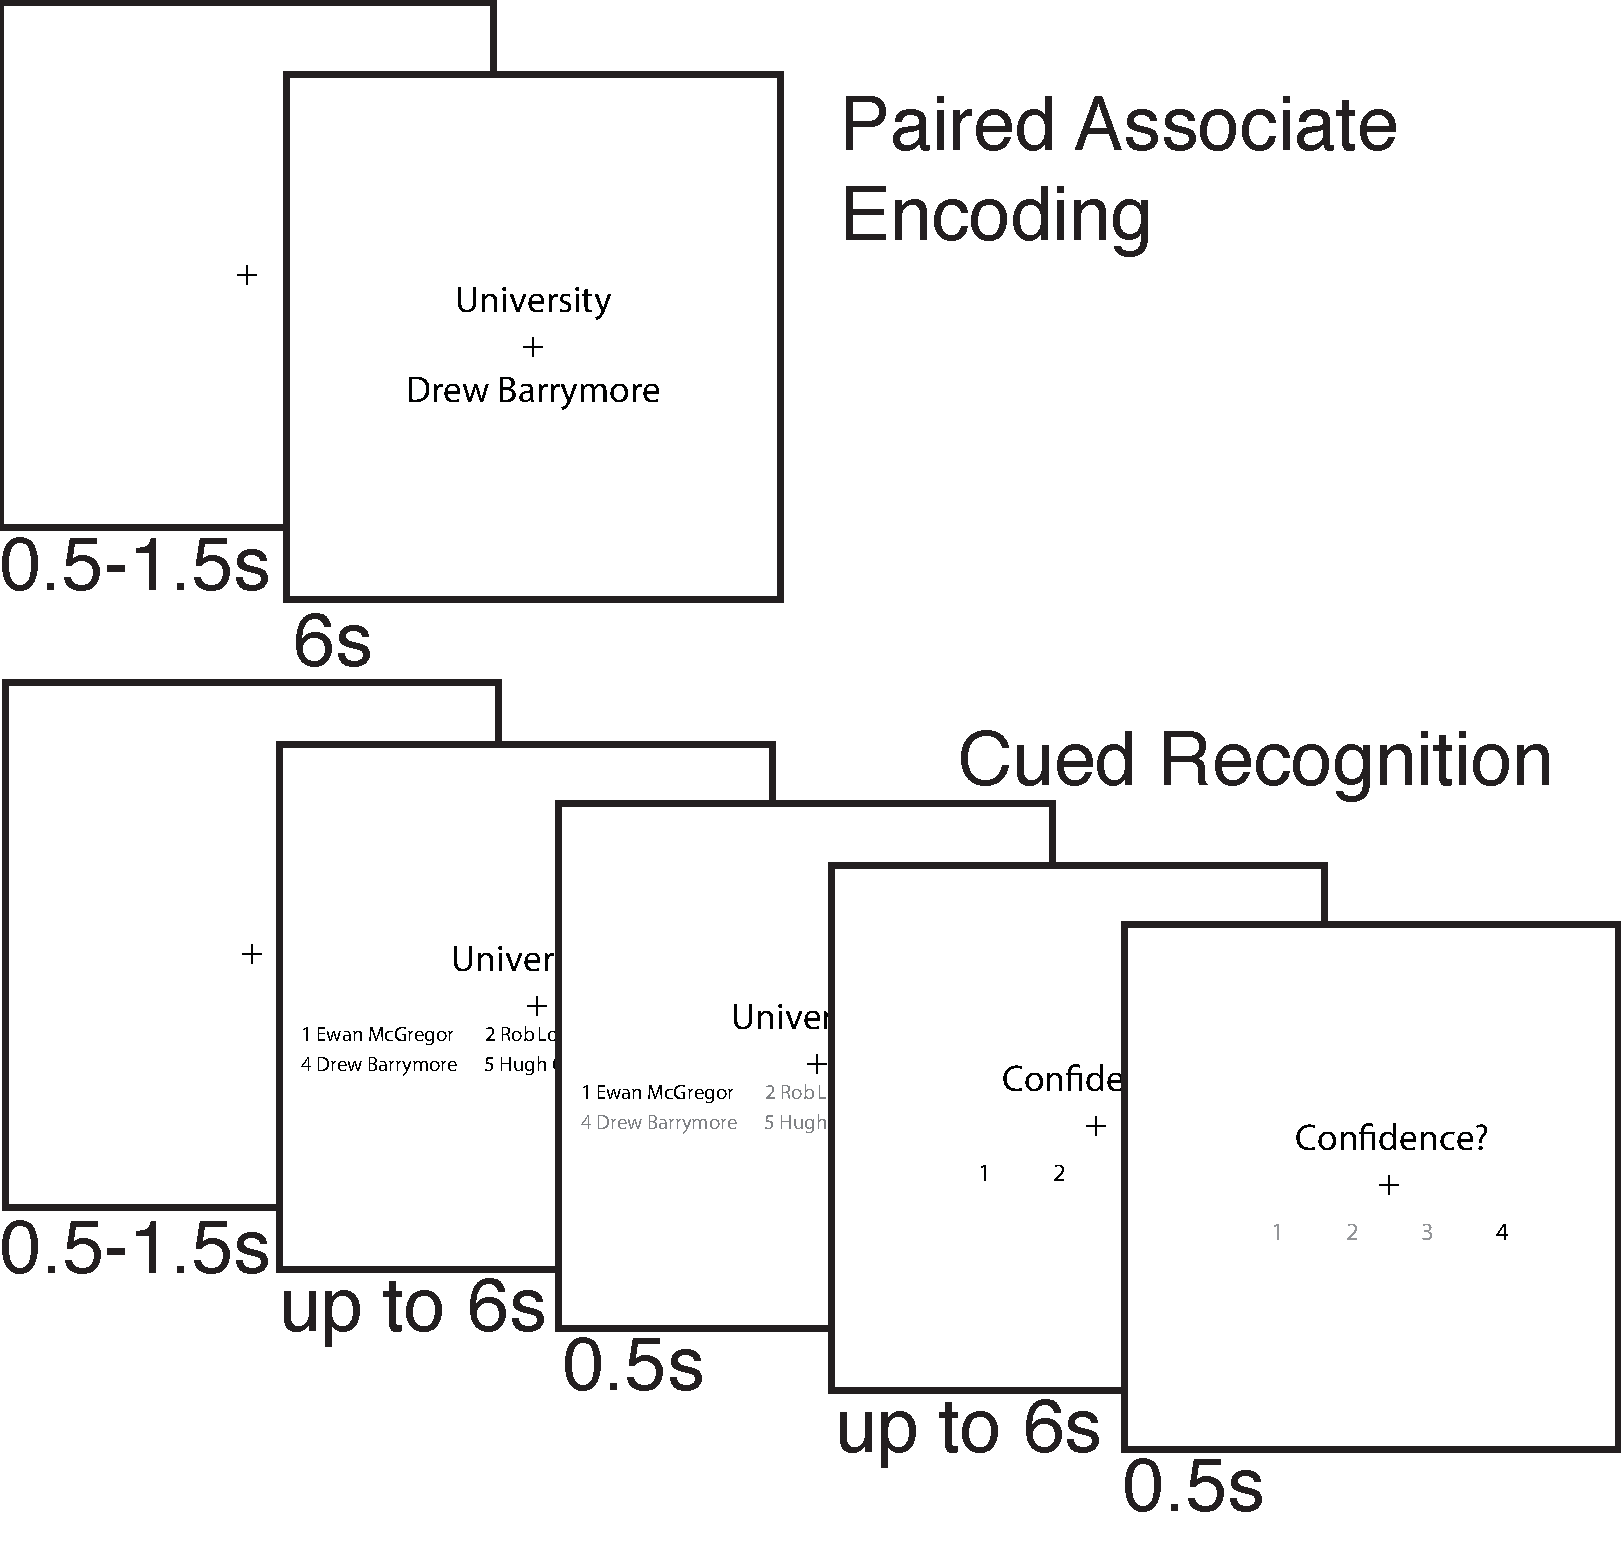
\includegraphics[width=.5\textwidth]{figs/deevTask.pdf}
	\caption[EEG Dependent Events Task]{
		Example stimuli and timing for Dependent Events paradigm adapted for EEG.  All trials had a uniform random inter-trial-interval (ITI) between 0.5s and 1.5s.  Timing was response driving for both cued recognition and confidence judgements.  After 6s a red warning message appeared directing the participant to make their selection.  Feedback was giving by turing grey the choice that was not selected during cued recognition and confidence judgements.  
	}
	\label{fig:deevTask}
\end{figure}



\subsection{Electrophysiological recordings}
A 128-channel HydroCel Geodesic Sensor Net (GSN 200, v. 2.1; Tucker, 1993) was used to measure the EEG at the scalp using a central vertex reference (Cz) with a sampling rate of 250 Hz and a low-pass hardware filter at 100 Hz. The net was connected to a DC-coupled, high-input impedance amplifier (200 M$\Omega$, Net AmpsTM; Electrical Geodesics, Inc., Eugene, OR) and recordings were made using the Net Station application. The electrodes were adjusted until impedance measurements were less than 40 k$\Omega$.

All EEG data was taken from retrieval trials where all processing steps and analyses were done in MATLAB using in-house scripts (mat-mvm, n.d.) and the FieldTrip toolbox \cite{OostenveldFriesMarisEtAl11}. A high-pass filter at 0.1 Hz, low-pass filter at 100 Hz, and a notch filter from 59--61 Hz were applied to the data.  ICA artifact removal targeting blinks, and movement artifacts was done on the continuous (i.e. pre-epoched) EEG data after removal of large artifacts through coarse visual inspection.  A semi-automated approach to artifact estimation and detection was done using the SASICA plugin ported for FieldTrip data structures, and methods described in \textcite{ChaumonBishopBusch15}.  After ICA artifact removal, each cued recognition trial was epoched in two ways: stimulus locked (SL) and response locked (RL).  SL epochs were 5000 ms segments, 1 s before the onset of the cue and target array, and 4 s after. RL epochs were also 5000 ms segements, 4 s before target response was made and 1 s after.  Fieldtrips's automatic artifact detection was used to reject particularly noisy epochs as determined by a $z$-score threshold of 20, as well as those that exceed an amplitude of $\pm$200 $\mu$V or a maximum change in amplitude of 200 $\mu$V. 

On average across subjects and conditions (i.e. both stimulus and response locked open and closed-loop trials) $37\pm4$(standard deviation) percent of trials were removed due to potential artifacts; there were no significant differences between conditions within epoch type in the number of removed trials.  After artifact rejection the data were referenced to the average of all channels, after which wavelet based time frequency decompositions were done.

\subsubsection{Spectral Analysis}
\label{sec:deevSpecAnal}
The spectral decomposition was performed using a set of 71 Morlet wavelets that were equally spaced in 0.67 Hz intervals from 3 to 50 Hz. Each wavelet had a width that was 4 times the period of its center frequency. The power, i.e., the squared magnitude of each complex coefficient, was then computed for every 40 ms time bin within the extracted time window. In total, the spectral decomposition transformed each of the time bins of a trial into the power values of 71 frequency bands for each of the 128 electrodes.  For each stimulus locked (SL) trial, power estimates after the response time were nulled out and were not figured into condition averages.  Similarly, for each response locked (RL) trial power estimates before the onset of the stimulus were also nulled out.  Each trial, both SL and RL, were then baseline corrected by $z$-scoring the full trial length based on a a given trial's pre-stimulus mean and standard deviation from time window between -300 ms to -100 ms relative to cue-target array onset.  

EEG results were analyzed according to the difference between open and closed-loop conditions.  To achieve this, $time \times electrode$ clusters were determined across subjects for each a-priori defined frequency band using a cluster based permutation test \cite{MarisOostenveld07}.  Frequency data were first averaged over a the defined frequency bands: 3-8 Hz for theta, 8-12 Hz for alpha and 12-30 Hz beta.  These data were then analyzed across all electrodes except the 4 surrounding the eyes, and across the time window of 500 to 3000 ms relative to the cue-target array onset in the stimulus locked epochs, and -3000 ms to -500 ms relative to the button press for a given trial in response locked epochs.  Clustering was done by performing a $t$-test comparing open and closed-loop conditions within each time/electrode bin across subjects for each of the target frequency ranges (theta, alpha and beta).  These $t$-values were then thresholded at $p<.05$, and clustered together based on spatial and temporal adjacency.   Cluster significance was calculated using a monte-carlo style permutation test of the summed $t$-values within a given cluster.  Each observed cluster was subject to 500 random permutations of condition labels where its significance was estimated by the proportion of random permutations which yielded clusters that had a summed $t$-value as large or larger than the observed cluster.

\subsubsection{Representation Similarity Analysis}
\label{sec:deevRSA}
The Representation Similarity Analysis (RSA), was motivated by the non-target reactivation seen in \textcite{HornerBisbyBushEtAl15} and was based on the methods originally developed by \textcite{KriegeskorteMurBandettini08}.  The underlying structure used in the RSA was based on individual retrieval trials within a given event and was done in two ways.  The first was the standard correlation approach where a similarity matrix was constructed by correlating the full $time \times frequency \times electrode$ matrix, splayed out to a single vector, pairwise with each retrieval trial within a given event.  Ideally this results in a 6x6 matrix with all 6 retrieval trials per event correlated with each other, however some retrieval trials were removed due to the presence of artifacts and therefore all events with more then 3 intact retrieval trials were used in the RSA.  The off diagonal $R$-values in this matrix were then converted to $z$-values using the inverse hyperbolic tangent, and averaged to achieve a single `similarity' measure across retrieval trials for a given event.  These were then averaged across condition with the prediction that more non-target reactivation would manifest in a higher similarity value averaged across events within a given condition.

The underlying structure used in the RSA was based on individual retrieval trials within a given event.  We adapted the RSA method to our data by using the measuring pairwise variance between trials within a given event to determine the `dissimilarity' of a given set of retrieval trials, i.e. the larger the variance across retrieval trials from a given event the more dissimilar the set of retrieval trails are.  Specifically, the pairwise variance across all retrieval trials within a given event was calculated for each significant $time \times frequency \times electrode$ bin.  This was then averaged across a-prior frequency bands (i.e. 3-8 Hz for theta, 8-12 Hz for alpha and 12-30 Hz beta), then averaged within conditions (closed-loop and open-loop) ultimately yielding a $time \times electrode$ matrix of dissimilarity per condition for each subject. This matrix was then analyzed using to the same non-parametric cluster statistics described above to determine significant differences between conditions clustered in time and space for each frequency band.  




\section{Results}\label{sec:results}

\subsection{Computational Model Results}\label{sec:compresults}

Overall model performance was good for both closed and open-loop events.  Accuracy of cued recall in the network was well above chance (1 of out 100 possible unit group patterns used to determine Name Error, or more conservatively 1 out 36 possible patterns used in the training) in all cue-target types for both conditions, shown in Figure \ref{fig:netDep}A.  This assures that the model was learning the paired associates patterns sufficiently in both conditions, and performing as expected. Closed-loop events did show a higher average accuracy compared to open-loop events across network runs ($\mu=0.14\pm0.06$ 95\% confidence), with the largest difference being when the object or animal elements were the retrieval target, similar to results from \textcite{HornerBisbyBushEtAl15}.  

\begin{figure}
    \begin{center}
	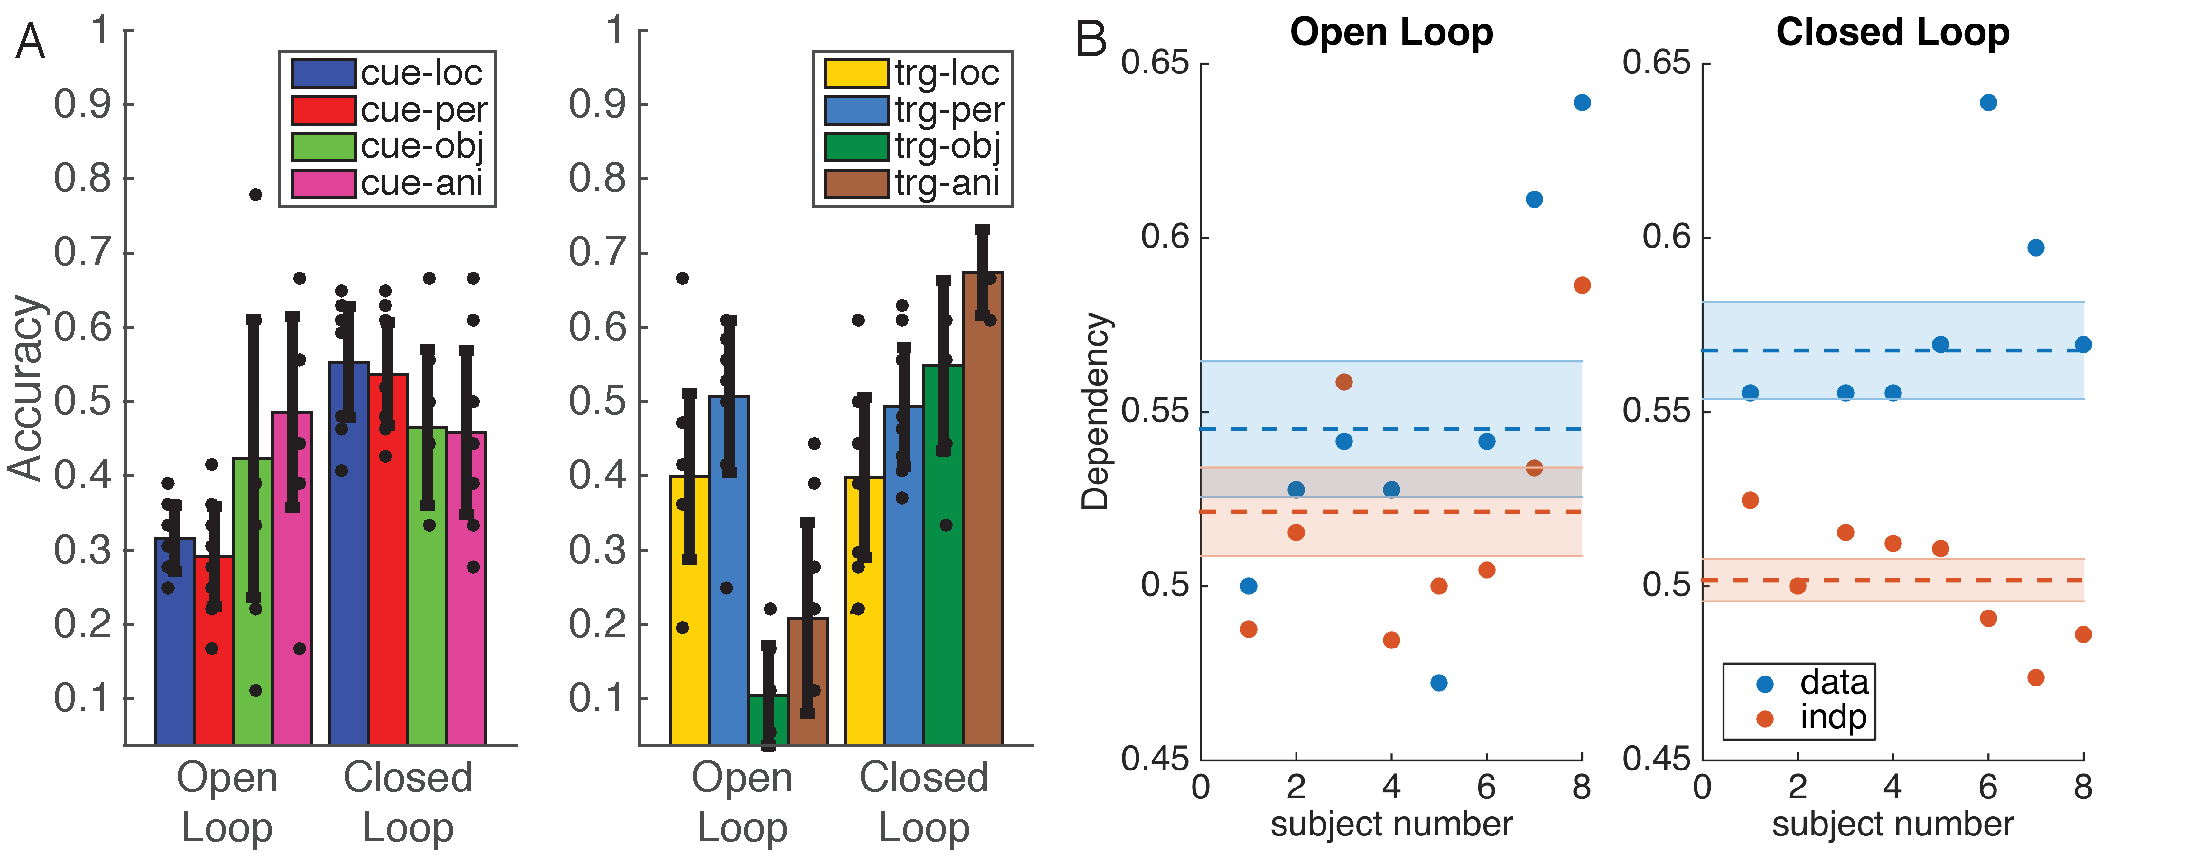
\includegraphics[width=\textwidth]{figs/netDep.pdf}
    \end{center}
      \caption[Open vs. Close Loop Performance]{
       \emph{(A)} Name Error assessed cued retrieval accuracy for all cue-targ and targ-cue combinations, averaged across network runs, within conditions. Black dots show individual network runs with unique random weight initialization balanced across encoding orders.  Error bars show 95\% confidence intervals.  \emph{(B)} Dependency assuming underlying event structure (labeled `data') and assuming all cue-targ trial types are independent (labeled `indp'), broken down by condition.  Horizontal axis shows individual network runs.  Dash lines show mean across network runs, and error bars show 95\% confidence intervals.
	}
     \label{fig:netDep}
\end{figure}

To validate the addition of attentional modulation to the Theta-Phase model a comparison was made between its performance and results from the Dependent Events paradigm%, shown in Figure \ref{fig:deev_neuroimg}
.  The first critical comparison was the Dependency difference between open and closed-loop events, with the anticipation of closed-loop events having greater within event Dependency as compared to open-loop events.  The second was the non-target reactivation difference with the anticipation that closed-loop events would shown greater non-target reactivation as compared to open-loop events.

\subsection{Condition Differences in Dependency}
As shown in Figure \ref{fig:netDep}B, Dependency was significantly greater than the Independent model for closed-loop events (paired difference within model runs: $\mu=0.07\pm0.04$ 95\% confidence, $t(7)=3.76,p<0.01$), and not different for open-loop events ($\mu=0.02\pm0.03, t(7)=1.82,p=0.1$).  The interaction between condition differences and Independent model was also significant ($t(7)=2.84,p<0.05$), with the difference between closed-loop Dependency and its Independent model being greater than the difference between open-loop Dependency and its Independent model.

It should be noted that the relatively low levels of Dependency witnessed in the network's performance compared to the original study's behavioral results %shown in \ref{fig:deev_neuroimg} 
can be attributed to the relatively small number of training epochs the network was subject to.  When a larger number of epochs (i.e. more then 3) are run, the difference between closed-loop Dependency and its Independent model goes away, however the accuracy level increases.  This suggests that the network is over-learning the representations, pushing accuracy to ceiling, and thus washing out the effects of Dependency.



\begin{figure}
    \begin{center}
	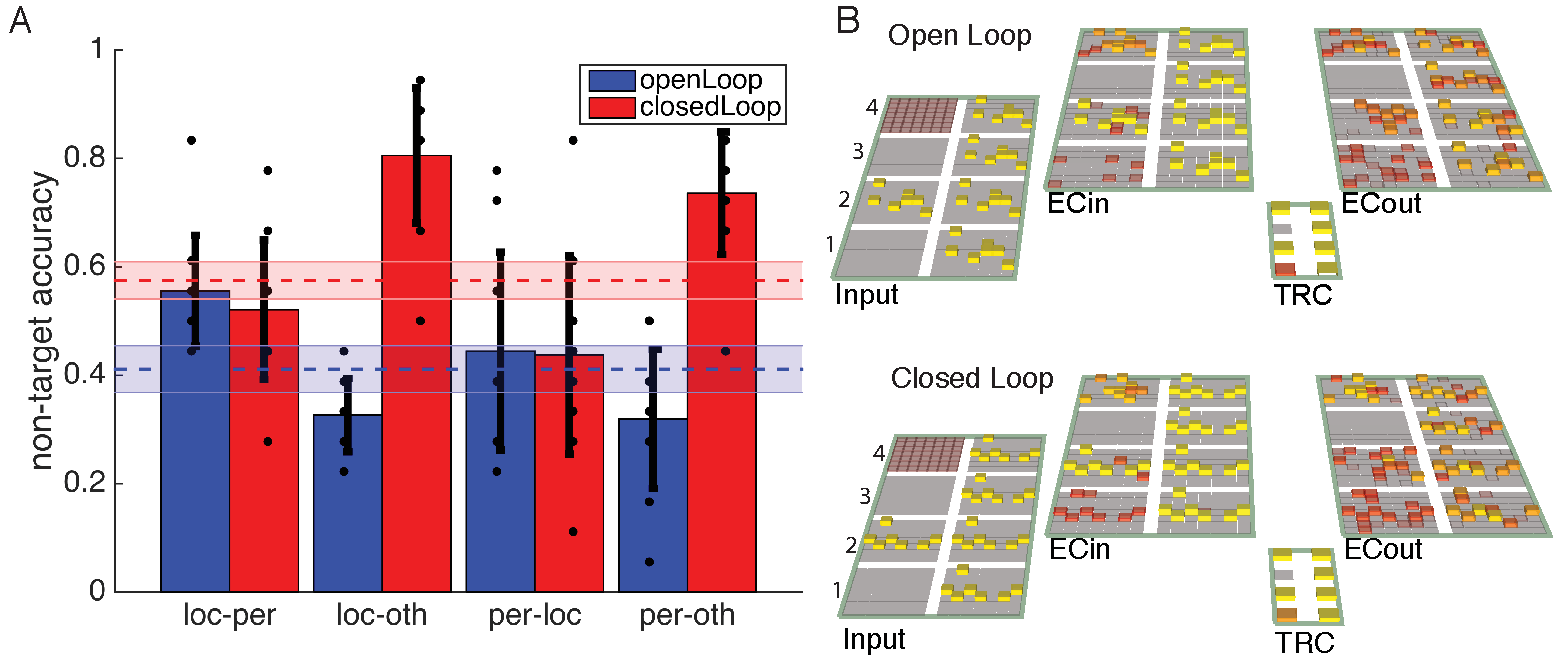
\includegraphics[width=\textwidth]{figs/depNonTarg_edit.pdf}
    \end{center}
      \caption[Non Target Reactivation]{
       \emph{(A)} Name Error accuracy for non-target reactivation in open-loop and closed-loop events.  The horizontal axis labels correspond to the cue and target respectively, and the non-target element is the one not listed in the label.  For example `loc-per' indicates a location cue and person target trial, and therefore the non-target element is either object or animal depending on the encoding paris for the given event.  The 'oth' label corresponds to either the object or animal element again depending on the corresponding encoding pairs for the given event.  Note, non-target accuracy was not assessed for object or animal elements as cues, as open-loop events have no corresponding non-target element in these cases, and would be a biased comparison with closed-loop events which do. Black dots indicate individual network runs with different training orders (see section \ref{sec:TestProc}), red bars are closed-loop and blue bars are open-loop, dash lines are means across all cue-targ trial types, and error bars are 95\% confidence intervals. \emph{(B)} Example cued retrieval trials from open-loop (top) and closed-loop (bottom) events.  Both show a retrieval trial with a person cue (unit group 2, as numbered to the left of the Input layers), and a animal target (unit group 4), and a location non-target (unit group 1).  TRC shows bottom-up (person and animal unit groups) as well as hippocampal driven (Location unit group) modulation of thalamic gate.
	}
     \label{fig:netNonTarg}
\end{figure}


\subsection{Condition Differences in Non-Target Reactivation}
As shown in Figure \ref{fig:netNonTarg}A, successful non-target reactivation, as assessed through Name Error, was significantly greater in the closed-loop condition compared to the open-loop.  Interestingly this difference was most pronounced in the retrieval trials in which the `other' (or object/animal) stimulus dimension was the target of the cued retrieval.  This implies that in open-loop trials, the network was less likely to successfully reactivate  the location or person stimulus elements when attempting to retrieve the animal/object elements.  This can be seen in Figure \ref{fig:netNonTarg}B where cued retrieval is shown for an example open-loop event on top and a closed-loop event on bottom.  Both examples are showing a retrieval trial where the cue element is person (unit group 2, numbering from lower left proceeding up), and the target element is animal (unit group 4), and the non-target element is location (unit group 1).  The relatively lower TRC activation in the non-target element for the open-loop retrieval compared to the closed-loop quantitatively shows the reduced non-target reactivation.  Similarly, the qualitative activity in the closed-loop EC in and out non-target unit group is more complete and closer to the correct pattern as compared to the open-loop activity.


\subsection{Behavioral Results}\label{sec:eegresults}


\begin{figure}
	\begin{center}
		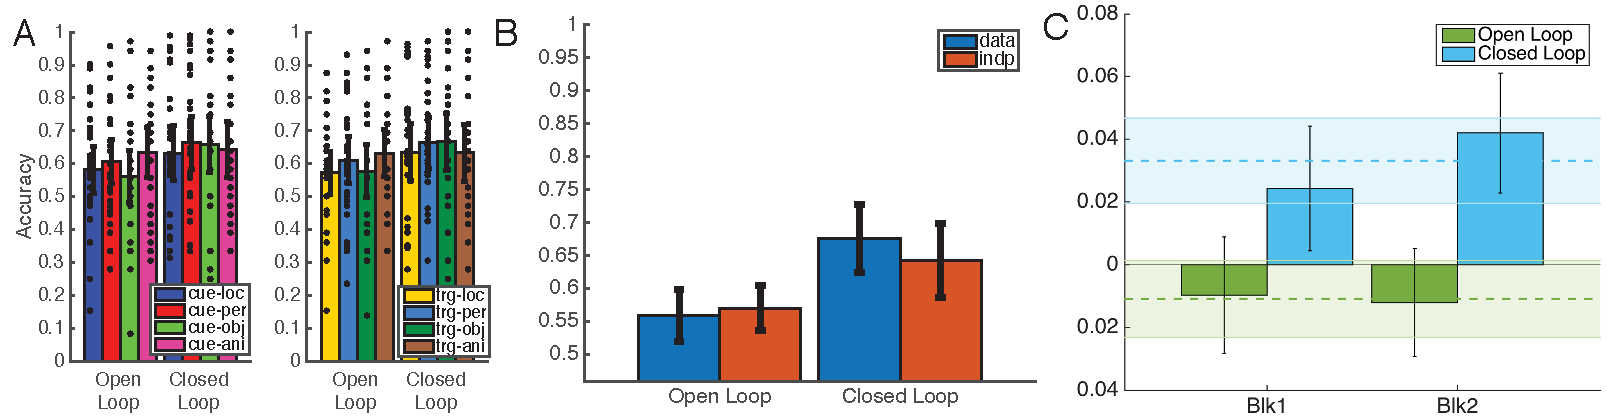
\includegraphics[width=\textwidth]{figs/deevEEGBeh_edit.pdf}
	\end{center}
	\caption[EEG Dependent Events Behavior]{
		\emph{(A)} Cued recognition accuracy for all cue-targ and targ-cue combinations, averaged across participants, within conditions. Black dots show individuals' performance.  Error bars show 95\% confidence intervals. 
		\emph{(B)} Average Dependency over subjects for both open-loop and closed-loop conditions.  Blue bars show Dependency assuming underlying event structure referred to as `data', and red bars are assuming all cue-targ trial types are independent referred to as `indp'. Error bars show 95\% confidence intervals. 
		\emph{(C)} Dependency difference as a function of block.   Dash lines show mean across blocks, and error bars show 95\% confidence intervals.
	}
	\label{fig:deevEEGBeh}
\end{figure}


Behavioral results, as seen in Figure \ref{fig:deevEEGBeh}, show a significant difference in accuracy between closed-loop and open-loop conditions (closed-loop minus open-loop: $\mu=0.05\pm0.03$ 95\% confidence, $t(27)=3.92, p<0.001$), similar to \textcite{HornerBisbyBushEtAl15} and the neural network simulation results.  Retrieval confidence was also significantly higher in the closed-loop trials as compared with open-loop (closed-loop confidence minus open-loop confidence: $\mu=0.21\pm0.1 t(27)=4.34, p<0.001$).  Similarly, average retrieval confidence was highly correlated with accuracy across subjects ($r=0.83,p<0.001$).

Critically, there was significant difference between Dependency and the Independent model in the closed-loop condition ($\mu=0.03\pm0.01, t(27)=4.91, p<0.001$), and not in the open-loop condition ($\mu=-0.01\pm0.01, t(27)=-1.78, p=0.09$), and there was also a significant interaction in Dependency by condition, with the difference between closed-loop Dependency and its Independent model being greater then the difference between the open-loop Dependency and its Independent model ($\mu=0.04\pm0.02, t(27)=4.93, p<0.001$).  There were significant differences for accuracy between blocks for closed-loop events (block 1 minus block 2: $\mu=-0.10\pm0.07, t(27)=-2.74, p<0.05$) and Dependency ($\mu=-0.07\pm0.06, t(27)=-2.68, p<0.05$).  Interestingly, these block effects are in the opposite direction as would be predicted from proactive interference, where memory performance progressively gets worse over the blocks.  Similarly, the difference between closed-loop Dependency and its Independent model was significant when considered within each block separately (block 1: $\mu=0.03\pm0.02, t(27)=2.51, p<0.05$; block 2: $\mu=0.04\pm0.02, t(27)=4.49, p<0.001$), however there was no significant interaction in this difference across blocks ($\mu=-0.02\pm0.03, t(27)=-1.32, p=0.2$).


\subsection{EEG Results}\label{sec:eegresults}



\begin{figure}
	\begin{center}
		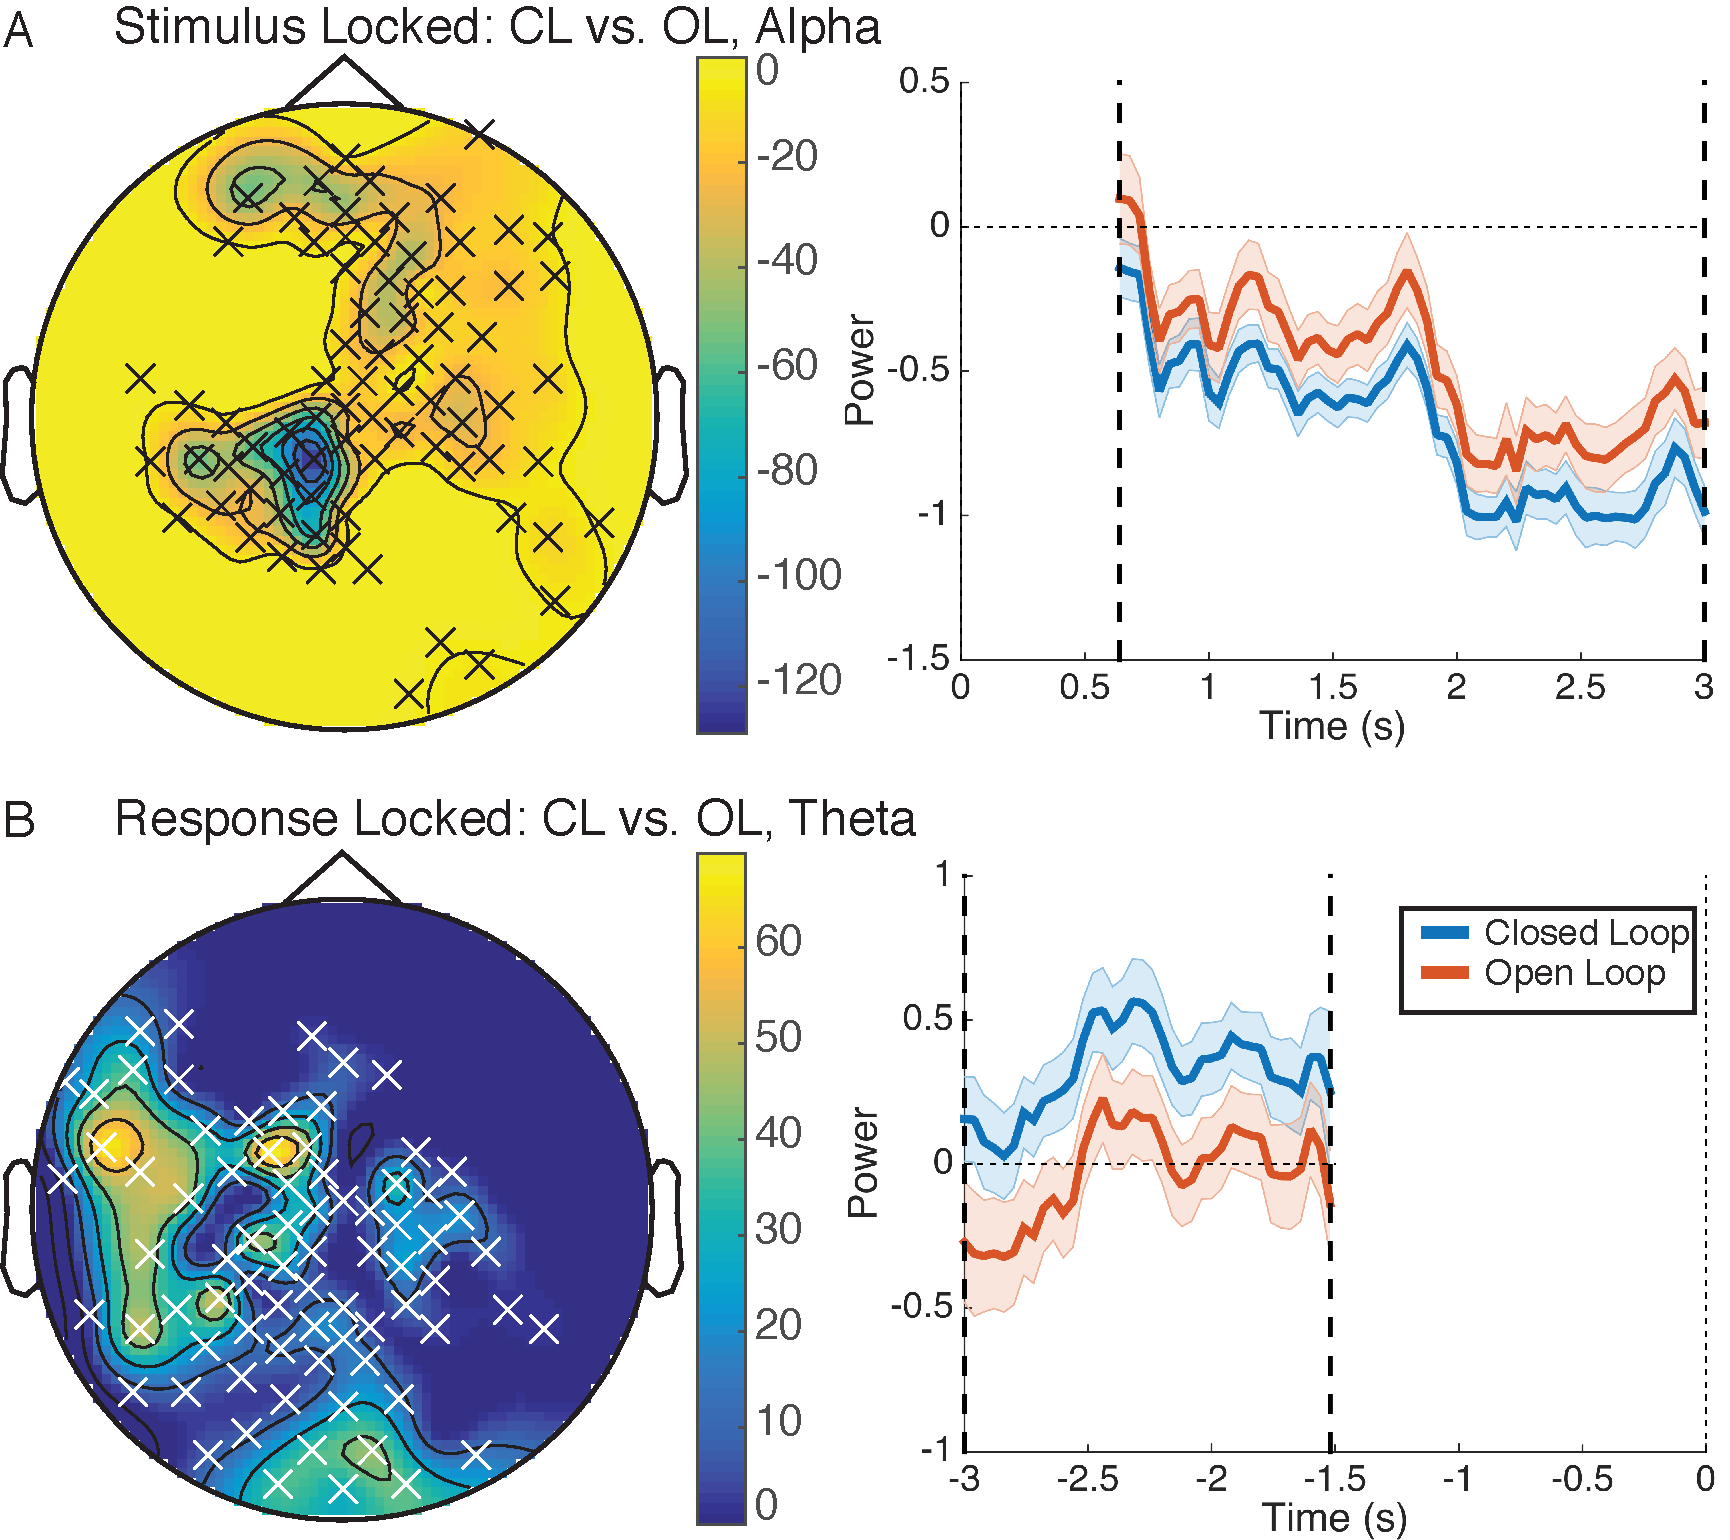
\includegraphics[width=.9\textwidth]{figs/deevPowerClusters_edit.pdf}
	\end{center}
	\caption[Closed vs. Open Loop EEG Clusters]{
		\emph{(A)} Cluster of alpha power showing significant difference between closed vs. closed-loop events, i.e here open-loop events showed more power as compared to closed-loop events for the highlighted $time \times electrode$ bins within the alpha band.  Cluster significant between 640 ms to 3000 ms relative to onset of cue-target array, and in the highlighted electrodes.
		\emph{(B)} Cluster of theta power showing significant difference between closed vs. closed-loop events.  Here closed-loop events showed more power compared to open-loop events in the highlighted $time \times electrode$ bins within the alpha band.  These were the only two clusters to meet the $p<0.05$ criteria within theta, alpha, and beta frequency bands for both stimulus locked and response locked epochs.  Topography on the left shows summed t-values over time with significance determined by permutation test, and on the right shows the average power within the significant electrodes with closed-loop shown in blue and open-loop shown in red.  The significant time window is bounded by the large dashed lines.
		%\emph{(C)} Average power extracted from the frequency band specific clusters.  Plotted on the left is the average theta power extracted from the theta defined cluster (i.e. Fig. \ref{fig:deevPowerClusters}B) as a function of within event retrieval attempt.  Plotted on the right is the average alpha power extracted from the alpha defined cluster (Fig. \ref{fig:deevPowerClusters}A). Dashed lines show the with-in subject difference of closed-loop vs. open-loop, and shaded error shows standard error.
	}
	\label{fig:deevPowerClusters}
\end{figure}

\subsection{Closed vs. Open Loop EEG Clusters}
\label{sec:deevCLvOL}
Condition differences between open and closed-loop EEG time frequency was assessed using the cluster based approach described in \textcite{MarisOostenveld07}, with a-priori defined frequency bands in the theta (3 to 8 Hz), alpha (8 to 12 Hz), and beta (12 to 30Hz) bands, and temporal windows between 500 and 3000 ms relative to cue-target onset (referred to as Stimulus Locked), and -3000 to -500 ms relative to button press (referred to as Response Locked).  Critically, open and closed-loop trials for this analysis were sub-selected to only include trials where the target item was correctly identified, this yielded Stimulus Locked condition trial counts: closed-loop $\mu=81\pm19$ 95\% confidence interval over subjects, open-loop $\mu=72\pm15;$ and Response Locked condition trial counts: closed-loop $\mu=88\pm18$, and open-loop $\mu=79\pm15$.  This subselection highlights the fact that any differences are not driven by accuracy between the conditions (however very similar effects were also found using all trials). 

Two clusters were found meeting the $p<0.05$ permutation significance level, shown in Figure \ref{fig:deevPowerClusters}.  The first was found in the alpha band from 640 to 3000 ms Stimulus Locked, and showed a greater decrease in baseline corrected closed-loop power as compared to open-loop.  The majority of the $t$-value mass was in the central posterior electrodes and spanned towards right-central anterior.  The second significant cluster was found in the theta band from -3000 to -1520 ms Response Locked, and showed a greater increase in baseline corrected closed-loop power as compared to open-loop events.  Its bulk of $t$-value mass was in left anterior electrodes, and spanned toward central posterior electrodes. 


%\subsubsection{Change in Power over Retrieval Attempts}
%\label{sec:deevPwrXBlk}
%To try and estimate the impact of how the strength of reactivation changes over retrieval attempts, the average power from the defining frequency band was extracted for each retrieval trial in the two clusters shown in Figure \ref{fig:deevPowerClusters}, i.e. alpha (8 to 12 Hz) power extracted from the cluster shown in. \ref{fig:deevPowerClusters}A, and theta (3 to 8 Hz) from \ref{fig:deevPowerClusters}B.  The average power over within-event retrieval attempts is shown in Figure \ref{fig:deevPowerClusters}C, with the closed-loop condition in the red line, the open-loop condition in green, and the within subject difference shown in the dashed line.  Two separate trial-level mixed effects statistical models were run using the power extracted from each of these clusters as the dependent variable, and fixed effects were estimated for: condition (closed-loop vs. open-loop), and ordinal retrieval attempt number (within event retrieval attempt 1 to 6) using a linear contrast code.  Random effects intercepts were estimated for subject, block, and linear retrieval attempt.  

%In both the theta and alpha models a significant main effect for condition was found, as would be expected from the cluster definition (theta: $t=2.81, p<0.005$, alpha: $t=-3.50,p<0.001$).  The theta model showed no significant effects by block, or interaction.  The alpha model showed a marginal main effect for the linear retrieval attempt predictor ($t=-1.79,p=0.07$), suggesting across conditions there was a linear decrease in alpha power over retrieval attempts, however there was no significant interaction.


\subsection{Representation Similarity Analysis}
In an attempt to test for non-target reactivation a Representation Similarity Analysis was done across retrieval attempts within a given event.  The interpretation of this analysis is that events with more non-target reactivation across the various cued recognition retrieval attempts would show more similarity in their EEG time frequency topography.  The first approach, see Section \ref{sec:deevSpecAnal} for a more complete description, tried to maintain as much alignment with standard RSA as possible, by doing correlations using the full frequency spectrum (3 to 50 Hz), and the full time window (500 ms to 3000 ms for Stimulus Locked epochs, and -3000 ms to -500 ms Response Locked).  Averaging pairwise correlations across all retrieval attempts within a given event yielded a single measure of similarity for each event, which were then averaged into open and closed-loop conditions. No significant differences were found between open and closed-loop events for both stimulus locked and response locked epochs.  It is likely the full $time \times frequency \times electrode$ space is non-optimal for detecting these similarity differences, and in an attempt to narrow down this space a second approach was adopted to take advantage of the clustering methods used in the power analysis.

This second approach measured the variance across the 6 retrieval attempts within an event for each $time \times frequency \times electrode$ bin.  For example, the power estimate at time bin 0.4s, frequency bin 5 Hz, and electrode 128, is extracted for the 6 retrieval attempts in event 1.  The variance is then calculated over these 6 values, and put into a 3d matrix with the same dimensions as the original data.  Repeating this process for all $time \times frequency \times electrode$ bins yields a \emph{dissimilarity} measure for each bin in the full 3 dimensional matrix for a specific event.  Repeating this across events yields a maximum of 72 separate event matrixes, which are then averaged within each condition to get single open-loop matrix and single closed-loop matrix for each subject.  Using the clustering method described in Section \ref{sec:deevSpecAnal}, a permutation test was done looking for the $time \times electrode$ clusters for each frequency band that showed a significant difference between the open and closed-loop conditions.  This yielded two significant clusters from the Stimulus Locked data at the $p<0.05$ level as determined through a permutation test, see Figure \ref{fig:deevVarClusters}.  The first was in the theta band, showing more dissimilairty in the open-loop condition compared to the closed-loop (permutation significance $p<0.05$).  This cluster spanned from 2320 ms to 3000 ms, and the main bulk of the $t$-value mass was in the central posterior electrodes and spanned up to central anterior electrodes. The second was a alpha cluster, also showing more dissimilarity in the open-loop condition compared to the closed-loop.  This cluster spanned from 2560 ms to 3000 ms, and the bulk of the $t$-value mass started in right anterior electrodes and spread to virtually all electrodes. 

\begin{figure}
	\begin{center}
		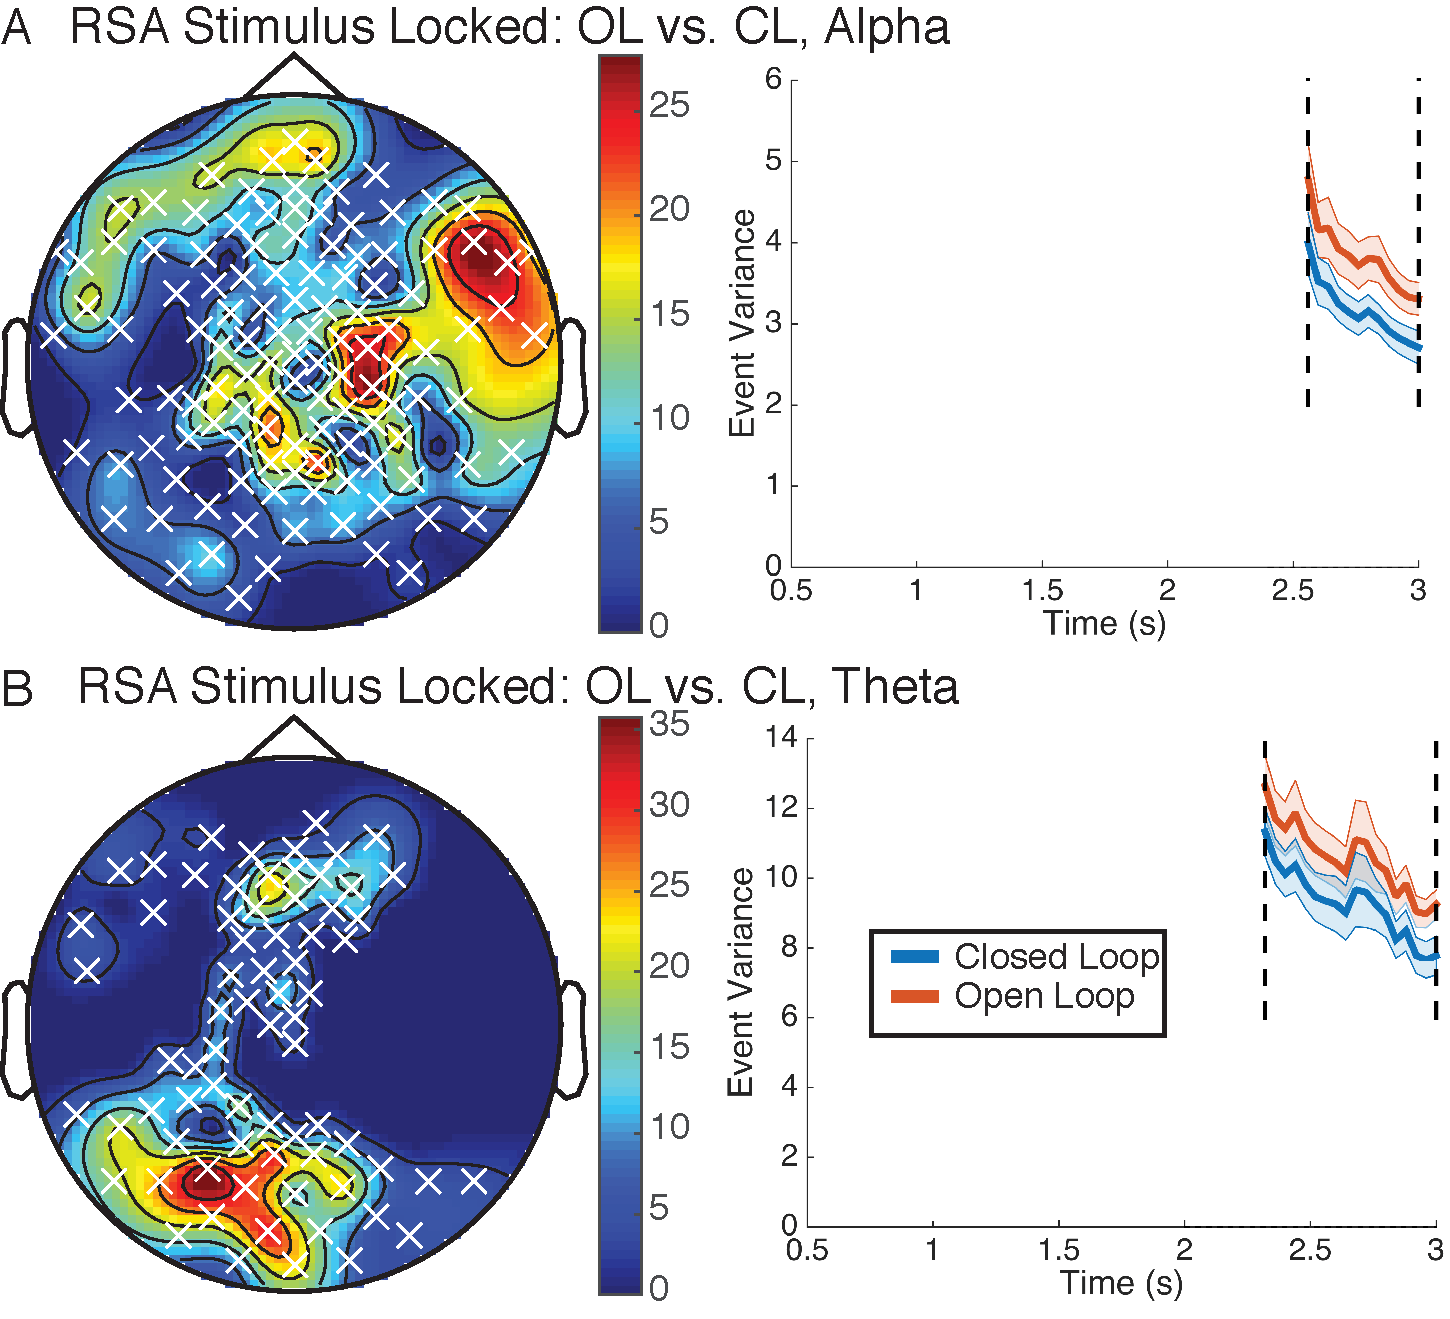
\includegraphics[width=.9\textwidth]{figs/deevVarClusters_edit.pdf}
	\end{center}
	\caption[Representation Dissimilarity EEG Clusters]{
		\emph{(A)} Cluster of representation variance difference between open-loop and closed-loop events in the alpha band.  Here open-loop events showed more within event variance as compared to closed-loop events for the highlighted $time \times electrode$ bins within the alpha (8 to 12 Hz) band.  Cluster significant from 2560 ms to 3000 ms relative to onset of cue-target array, and in the highlighted electrodes.
		\emph{(B)} Similar cluster for representation variance difference found in theta band.  Again, open-loop events showed more within event variance as compared to closed-loop events for the highlighted $time \times electrode$ bins, this time in the theta (3 to 8 Hz) band.  Cluster significant from 2320 to 3000 ms relative to onset of cue-target array.  These were the only two clusters to meet the $p<0.05$ criteria within theta, alpha, and beta frequency bands for both stimulus locked and response locked representation similarity analyses.   Topography on the left shows summed t-values over time with significance determined by permutation test, and on the right shows the average power within the significant electrodes with closed-loop shown in blue and open-loop shown in red.  The significant time window is bounded by the large dashed lines.
	}
	\label{fig:deevVarClusters}
\end{figure}







\section{Discussion}\label{sec:discussion}

Building from the theta-phase model \cite{KetzMorkondaOReilly13}, a mechanism supporting perceptual inhibition in service of long-term memory encoding was purposed.  This encoding mechanism in fact works through the successful retrieval of previously encoded information, further strengthening previous associations and binding them to new experiences. This comprehensive model of the hippocampus and surrounding cortex was then used to explore a multi-element memory paradigm shown to differentially engage the hippocampus, referred to as the Dependent Events paradigm.   Here, the mechanisms relating hippocampal reactivation to theta oscillations and attentional filtering to alpha oscillations provided explanatory power in understanding why different association structures lead to more pattern completion, i.e. closed-loop events, as compared to others, i.e. open-loop events. The results showed that repeated reactivation of information incidental to the current task, i.e. in the closed-loop events, strengthen the underlying association structure of those memories, while memory traces which didn't experience this reactivation, i.e.  open-loop events, showed more attentional filtering of cortical processing.  This filtering blocked reactivation of weaker associations, and instead strengthened only the cue-target associations.  The implications of this attentional selection process revealed a potential mechanism to explain the behavioral differences in the Dependent Events paradigm, and more generally provides a model of how retrieval processes can both strengthen are degrade associations depending on task goals as well as memory strength.

%summary exp1 and 2
These simulations were followed up with empirical studies testing the behavioral and EEG time frequency predictions derived from the simulations.  %The first was a direct replication of the Dependent Events paradigm, as designed by \citet{HornerBisbyBushEtAl15}, in the EEG domain.  The study looked to validate the prediction that increased hippocampal pattern completion would lead to increased cortical theta power.  Similarly, the predicted relationship between attentional filtering and alpha power was tested, where less memory reactivation manifests in higher alpha power. Finally, a separate behavioral study manipulated this relationship by modifying the standard Dependent Events paradigm to use bottom-up information to promote the reactivation of interfering associations.
Those results support the predictions of the computational model.  Specifically, it was found that theta oscillations increased for successful retrieval attempts which showed more reactivation of incidental, or `non-target', information as compared to retrieval attempts which did not.  Similarly, alpha power showed a greater decrease when retrieval reactivated more non-target information.  This reactivation process manifests as a behavioral change in `Dependency' between pairs of stimuli that shared an underlying association structure, referred to as `events'.  Here Dependency is measured as an increased probability of correctly retrieving all (or none) of the associated items, and the computational model predicted that more reactivation leads to greater Dependency.  This reactivation was also independently tested through a Representation Similarity Analysis (RSA).  Here, more similarity between retrieval attempts within a given event was shown to track with Dependency, and this increased similarity manifested itself in the theta and alpha frequency bands.




\subsection{Model of Thamlo-Cortical-Hippocampal Interactions}

What are the mechanisms in the model which support the differences witnessed between open and closed-loop association structures? The main cause of these condition differences likely stem from the model's ability to reactivate the non-target elements more so in the closed-loop compared to the open-loop condition.  This increased reactivation initially comes from the fact that each of the different event elements are studied together in the closed-loop events, allowing the network to be more likely to later reactivate those associations.  In contrast, because the open-loop events don't have the fully overlapping association structure that the closed loop events do, a given cue in the open-loop retrieval trial is only likely to reactivate its previously studied association which would be the target element of a given retrieval trial, and unable to reactivate the non-target element.  

By incorporating this thalamically mediated attentional modulation mechanism into the Theta-Phase model a new set of data can be captured by the simulations.  Further, a new handle on EEG time frequency signatures and the underlying thalamic mechanisms is in place for further testing.  Due to the motivating biology supporting this computational model, several hypothesis can now be generated regarding the relationship of neural oscillations and the Dependent events paradigm, or pattern completion and bottom-up attentional modulation more generally.  First, due to the greater Dependency and greater non-target reactivation witnessed in closed-loop events we can expect greater cortical theta power in the EEG time frequency signature.  This is due to the hippocampus driving cortex into pattern completion, as witnessed in the model at Entorhinal Cortex (EC) but assumed to also propagate out to distributed cortical regions that ultimately feed into EC.  The second major hypothesis is that cortical alpha power should inversely scale with the amount of attentional modulation used in the network, such that when the network's attentional modulation is high, EEG alpha power should be low.  

In general this work provides another perspective on the same mechanisms of the Sync/deSync model \cite{ParishHanslmayrBowman18}.  Here, we propose a specific thalamic mechanism responsible for the alpha dynamics witnessed in declarative memory processes and implement it in a rate coding neural network model.  This model, however, does not directly manifest alpha dynamics that can be directly measured, it only indirectly models them through the thalamo-coritical-hippocampal interactions.  \textcite{ParishHanslmayrBowman18}, use a spiking model to ellicit measures that are more directly related to the oscillatory dynamics that both their and our models are interested in.  Similarly, varying levels of detailed thalamo-cortical models provide solid ground for exploring the attention mechanisms proposed here \cite{HindriksvanPutten13, BeckerKnockRitterEtAl15}.   Future work can try and bridge this gap by including the spiking dynamics of the Sync/deSync model with the systems level mechanisms of our model.

\subsection{Behavioral and EEG Support}
The computational simulations explored in this work suggests that the hippocampus is driving cortex during retrieval more so in the closed-loop events compare to the open-loop, and the EEG time frequency clusters and Representation Similarity Analysis (RSA) witnessed in this study suggest this reactivation manifests in the theta and alpha bands.   Specifically, the closed-loop trials showed a greater increase in theta power from a fixation baseline as compared to the open-loop trials.  Conversely, in the alpha band there was a greater decrease in baseline corrected power for the closed-loop compared to the open-loop trials.  

The RSA results also support this relationship to alpha and theta power.  The clusters shown in Figure \ref{fig:deevVarClusters} illustrate that the open-loop condition shows more variance in EEG power over retrieval attempts within a given event as compared with the closed-loop condition, and that this variance is specific to the theta and alpha bands in the scalp topographies shown.  This reinforces the interpretation that closed-loop retrieval attempts are more likely to reactivate all elements within a given event, where the hippocampus drives cortex in theta band and turns off thalamo-cortical suppression in the alpha band.  

Its interesting to note that the alpha cluster was found in the Stimulus Locked epochs and the theta cluster was found in Response Locked.  This fits with the interpretation that alpha is more directly related to perceptual information while theta is related to the reactivation of previous experiences.  Here the difference in alpha power is locked to the input stimulus and sustains over the extent of the trial, suggesting that even before a strong retrieval has occurred some differences between closed and closed-loop events are present.  Conversely, theta differences are locked to the response, suggesting that once a sufficient amount of information has been retrieved a decision can be made.  This decision process is presumable happening in the latter half (i.e. -1500 to 0 ms) of the Response Locked epochs.

These results provide new insight into the Dependent Events paradigm, and helps illustrate the temporal dynamics that was not previously possible in the fMRI studies.  Specifically, the response locked theta effects and stimulus locked alpha effects both support the mechanism proposed by the computational model, and provide extra insight into the dynamics support the Dependent Events paradigm.    



\section{Conclusions}\label{sec:conclusions}

In this work we have proposed a model of thalamo-coritical-hippocampal interactions that makes specific hypothesis about the role and relative magnitudes of neural oscillations during declarative memory processes.  Within the Dependent Events paradigm, simulations show that this model captures broad EEG time frequency dynamics related to alpha and theta oscillations, and makes mechanistic predictions about how these oscillations relate to the underlying neural processes and their implications for cognitive level behavior.  An EEG study using the same paradigm replicated previous studies' behavioral results and showed similar patterns of oscillatory dynamics as predicted by the neural network model.  



\printbibliography
%
%
%\section{Supplemental}\label{sec:supp}
%
%\subsection{High vs. Low Confidence EEG Clusters}
%\label{sec:deevEEGConf}
%Here trials were selected based on the confidence ratings given for each retrieval attempt with the intention of capturing differences in EEG time frequency for Recollection vs. Familiarity based memory retrieval.  The same analysis approach used in the closed-loop vs. open-loop results was adopted for this confidence contrast (i.e. cluster based search in Stimulus Locked and Response Locked within theta, alpha and beta frequency bands).  All correctly retrieved trials with confidence rating less then 3 were assigned to the Low Confidence condition, and all correctly retrieved trials with confidence greater then 2 were assigned to the High Confidence condition (trial counts: low confidence correct $\mu=25\pm4$ 95\% confidence interval across subjects, high confidence correct $\mu=127\pm33$).  It should be noted that this difference in trial counts per condition should not impact the type 1 error rate of the cluster statistics as significance is calculated through a bootstrapped random permutation of condition labels across subjects.
%
%Figure \ref{fig:deevConfClusters} shows the only 3 clusters found using the $p<0.05$ criteria; all clusters were found in the Response Locked epochs.  The theta cluster showed a greater increase in power relative to baseline for the High Confidence condition compared to Low Confidence, had a temporal extent from -3000 ms to -680 ms Response Locked, and its $t$-value mass was centered in left posterior electrodes.  In contrast, the alpha cluster showed a greater decrease in power for the Low Confidence condition compared to High Confidence, had a temporal extent from -3000 ms  to -480 ms Response Locked, and its $t$-value mass was in central posterior electrodes.  Similarly the beta cluster showed a greater decrease in power for the Low Confidence condition compared to High Confidence, had a temporal extent from -3000 ms to -1600 ms Response Locked, and its $t$-value mass was centered in right anterior electrodes.
%
%
%\begin{figure}
%	\begin{center}
%		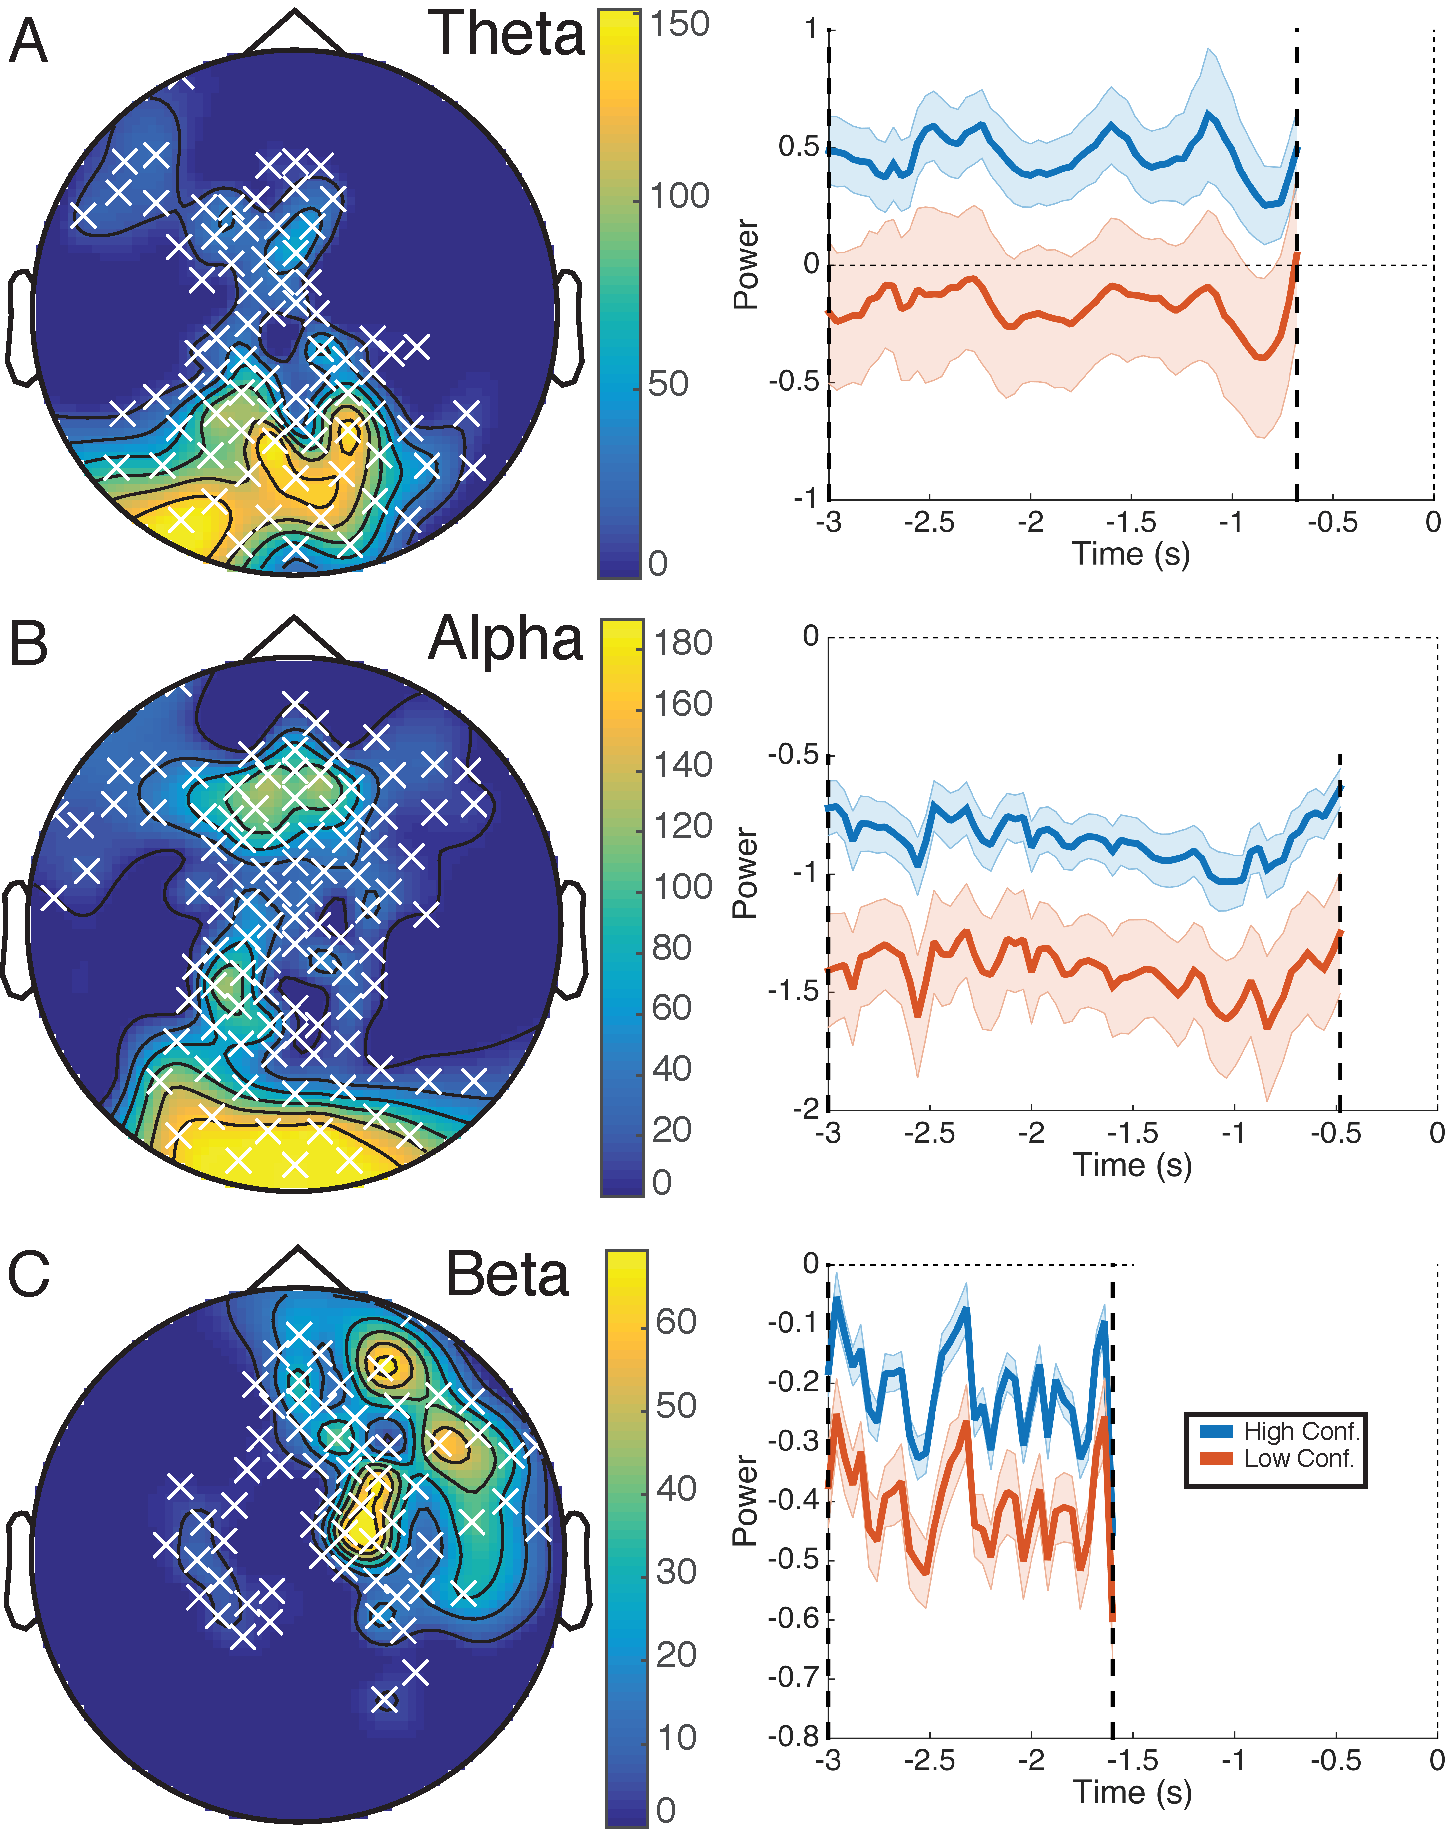
\includegraphics[width=.9\textwidth]{figs/deevConfClusters.pdf}
%	\end{center}
%	\caption[High vs. Low Confidence EEG Clusters]{
%		\emph{(A)} Clustered found for response locked power difference between High vs. Low Confidence correct retrieval trials in the theta band.  On the left is the summed $t$-values over time for significant electrodes, on the right is the average power across significant electrodes for High Confidence shown in blue and Low Confidence shown in red.  Large dashed lines show the boundaries of the significant temporal window.
%		\emph{(B)} Alpha cluster found for same contrast  as in A, here Low confidence trials show a greater decrease from baselined compared to high confidence trials.
%		\emph{(C)} Beta cluster found, with similar properties to the alpha cluster in B.  
%	}
%	\label{fig:deevConfClusters}
%\end{figure}
%
%
%
%
%\subsection{Theta-Phase Model}
%\label{sec:HippModelValidation}
%
%%add LEABRA details here?
%
%Input patterns were constructed, and memory retrieval performance measured, based on the slot topology in the EC layers (as highlighted in Figure~\ref{fig:depNet}).  This slot structure is intended to capture the modality segregation within EC, and within each slot we assume there is a {\em vocabulary} of different patterns, which reflect the representational repertoire within those modalities.  These vocabulary patterns were similarly used to estimate error within the networks' output by comparing, within a given slot, the output pattern of activation with all other vocabulary patterns.  If, for the given input pattern, the slots' output at the $\mathrm{EC}_{out}$ layer is closest to the vocabulary pattern it was trained on, it is considered correct, and otherwise considered incorrect.  This closest-pattern calculation is done across each of the slots for every input pattern, and if any slot shows an incorrect response the network output for that input pattern is counted as incorrect.  This measurement is referred to as \emph{Name Error} in the results section, and is thought to better represent the potential for clean up of hippocampal output as compared to more standard measures such as Sum Squared Error (SSE).    It also has the advantage of not requiring any further threshold or other parameterization.  It should be noted that this measure of error, compared to a SSE, deemphasizes single unit based errors in output in favor of an emphasis on distributed patterns of error across groups of units.
%
%
%\section{Attentional Modulation: Deep LEABRA}
%\label{appDeepLeabra}
%
%The `Deep LEABRA' framework currently being developed in the Emergent software is the initial explorations into the modeling of interactions between thalamic relay nuclei, and superficial vs. deep cortical layers \cite{OReillyWyatteRohrlich14}.  This framework proposes that the neocortex is composed of two separable networks: superficial and deep/thalamic. The superficial-layer network consists of neocortical layers 4, 2, and 3, across different brain areas.  The deep/thalamic network starts in each cortical area with the layer 5b intrinsic bursting (IB) neurons, which receive inputs from local superficial neurons and top-down projections from other areas, and provide strong driving feedforward input to higher-order thalamic nuclei. These 5IB neurons also project to deep layer 6 cortical-thalmic (6CT) neurons, which interconnects with the thalamus (which in turn projects back up to layer 4 of the superficial network and layer 6 in the deep network).  This connectivity is illustrated in Figure \ref{fig:attn_compute}.  The current work takes advantage of the biological referents and computational implementation of the Deep LEABRA frameworkm however, here it is used as a simple form of attentional modulation (and not a temporal learning mechanism as described in \textcite{OReillyWyatteRohrlich14}).  The minimal description of the components necessary for this implementation are described below.  
%
%The modulation of standard LEABRA unit activations (referred to as superficial units here) based the Deep LEABRA framework and the thalamic gating model described in \textcite{KetzJensenOReilly15} is carried out in two basic steps.  First, a Thalamic Relay Cell (TRC) unit receives input based on the threshold filtered output of some upstream units which have received its input from processing a given stimulus (in this case the hippocampus is providing this top-down modulation based on what is being retrieved).  These sending units, for a given TRC, are assumed to be the cortical thalamic projections from neocortical layers 5IB, 6CT \cite{ShermanGuillery06}, which reflect a thresholded filtering of superficial layer activity from both top-down and bottom-up sources. TRC activation dynamics are calculated in a similar manner to all LEABRA units, described in detail in \cite{KetzMorkondaOReilly13}, with the exception that its inputs are subject to an activation threshold of 0.1, and the weighted connections into and out of the TRC are not learned but instead remain fixed at 0.8.  
%
%Second, the TRC activation is used to calculate the attentional modulation that it sends to down stream superficial units.  The attentional modulation is implemented through a separate set of activations for receiving units that can be considered an attentional mask that gets applied.  This mask is the TRC activation normalized to a range between some pre-determined minimum and a maximum of 1.  The effective modulation of the receiving unit is simply the multiplication of this attentional mask, and the receiving units' net input.  Thus, where activations are strong in the mask, the corresponding superficial layer activations will remain strong, but where they are weaker, the superficial layer activations will be reduced.  This modulation process is hypothesized to be carried out by layer 6CT neurons  \cite{BortoneOlsenScanziani14,OlsenBortoneAdesnikEtAl12}.
%
%This multiplicitive modulation is based off previous mathematical models of attention that capture many of the effects relevant to the perception literature \cite{ReynoldsHeeger09,MontijnKlinkVanWezel12}.  Figure \ref{fig:attn_compute} shows how this framework captures the essential computations of the \textcite{ReynoldsHeeger09} model in different parts of the superficial and deep layer circuits.  Computationally, the TRC activations encode the attentional modulations of the superficial layer state. The attentional modulation signals cause the iterative constraint satisfaction process in the superficial network to focus on task-relevant information while down-regulating responses to irrelevant information, consistent with the abstract \textcite{ReynoldsHeeger09} mode.  Its important to note that this process can work in both a top-down (shown in \ref{fig:attn_compute}) and bottom-up fashion. Biologically, the layer 6CT neurons are known to exhibit a multiplicative influence over firing of superficial-layer neurons, in a manner consistent with the \textcite{ReynoldsHeeger09} model \cite{BortoneOlsenScanziani14,OlsenBortoneAdesnikEtAl12}. 
%
%
%\begin{figure}
%  \centering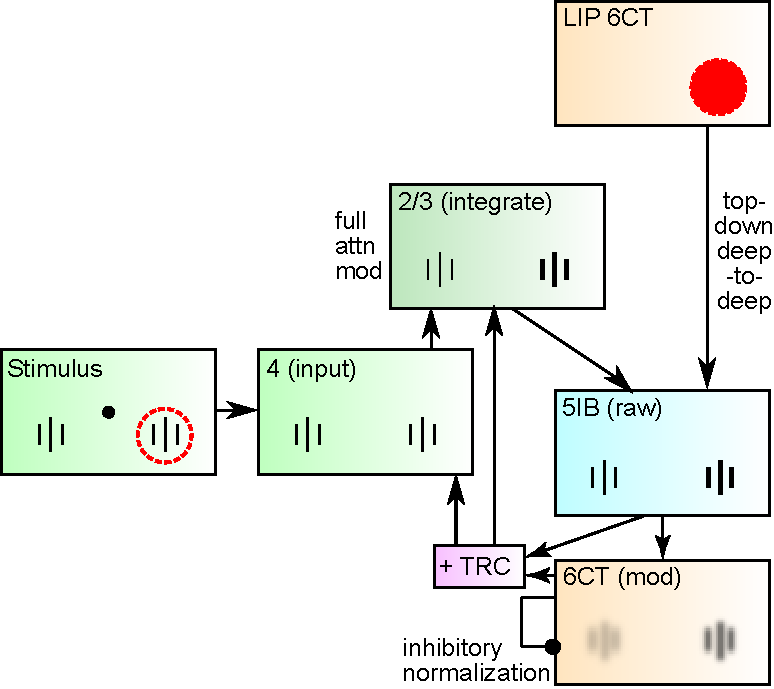
\includegraphics[width=.75\textwidth]{figs/fig_deepleabra_attn_compute.pdf}
%  \caption[Signal Flow Through Cortical Layers in Deep LEABRA]{\small How attentional modulation is computed in response to a top-down attentional focus.  Layer 4 receives bottom-up sensory input, which then drives superficial layers (2/3), which initially do not reflect the attentional modulation (not shown).  The deep layer 5 Intrinsic Bursting (5IB) neurons integrate deep-to-deep top-down attentional inputs plus the local stimulus features from 2/3, to produce a {\em raw} deep output, prior to the contextual normalization process.  Layer 6 Cortical-Thalamic (6CT) neurons then integrate this direct activation from 5IB, to produce, for the first time in the circuit, a properly renormalized multiplicative gain-field activation pattern, with surround inhibition both within the 6CT layer and further downstream in the  TRC circuit providing the renormalization process.  These 6CT activations then modulate (multiply) the superficial-layer activations to produce {\em both} an increase in the attended location, and a decrease for the unattended location, as shown.  
%  %In biological systems, this modulation also affects the layer 4 inputs (not shown) as well as 2/3, however, our model subsumes layer 4 into layer 2/3 neurons.
%  }
%  \label{fig:attn_compute}
%\end{figure}
%
%\subsection{Dependent Events Example Stimuli}
%\label{appStimuli}
%
%Below is an example set of events generated for the Dependent Events paradigm.  These stimuli were originally adapted from \textcite{HornerBisbyBushEtAl15}, where some original elements were removed due to British vs. American ubiquity, and replace with more common American elements.  The first 18 events are open loop, and the last 18 are closed loop with the appropriate balancing of object and animal stimuli.  
%
%
%\begin{longtable}{l|c|c|c|c} \small
%	\bfseries Event Number & \bfseries Location & \bfseries People & \bfseries Objects & \bfseries Animals  % specify table head 
%	\csvreader[head to column names]{evts.csv}{}% use head of csv as column names
%	{\\\hline\EventNumber & \Locations & \People & \Objects& \Animals}% specify your coloumns here
%\end{longtable}
%
%
%
\end{document}
